\documentclass[a4paper,12pt]{article}

% Load Packages
\usepackage{amsfonts,amsthm,amsopn}
\usepackage[psamsfonts]{amssymb}
\usepackage[cmex10]{amsmath}
\usepackage{amsmath}
\usepackage{enumitem}
\usepackage{natbib}
\usepackage[left=3cm,right=3cm,top=3cm,bottom=3cm]{geometry}
\usepackage[dvipsnames]{xcolor}
\usepackage[]{graphicx}
\usepackage{graphics}
\usepackage[bb=dsserif]{mathalpha}
\usepackage{bm}
\usepackage{subcaption}
\usepackage{booktabs}
\usepackage{rotating,tabularx}
\usepackage[font=small]{caption}
\usepackage{ulem}

\newcommand{\ex}{\mathbb{E}} % expectation
\newcommand{\ind}{\mathbb{1}}
\newcommand{\bfbeta}{\bm{\beta}} %bold beta coefficent

\setlength\parindent{0pt}
\renewcommand{\baselinestretch}{1.2}

\usepackage{xr}
\externaldocument{../paper/paper}
%\externaldocument{../paper/supplement}
\usepackage{hyperref}

% Start document
\begin{document}



\begin{center}
\underline{\Large\textbf{{Reply to reports on article JBES-P-2022-0567}}}\end{center}
\vspace{10pt}


First of all, we would like to thank the editor, the associate editor and the reviewers for their many comments and suggestions which were very helpful to improve the paper. In the revision, we have addressed all comments of the referees and have rewritten the paper accordingly.
%We also included an additional discussion of the extensions suggested by the referees that are closest to the original setup. Moreover, we have included additional details on the identification of the components in our multiplicative volatility model (cp. the beginning of Section 3.1) as we were not fully satisfied with the previous exposition.We also tweaked the simulation design to correspond more clearly to the setup discussed in the estimation section (cp. Section 7). 
%Finally, as requested, we have substantially shortened the paper to fit within the limit of 35 pages. This required to take all the proofs out of the paper and collect them in the supplementary material. In addition, we have rearranged the figures. In particular, the original Figures 2 and 3 are now contained in one figure. Similarly, the original Figures 6 and 7 are included in one figure. \\ 
Please find our point-by-point responses to the referees below. In our responses, we have indicated where alterations to the manuscript have been made to account for the points raised. Please also note that we have tried to put as much of the additional material as possible to the main body of the paper. However, to meet the 35 pages limit, we had to relegate the simulation study and parts of the additional material (including the multiple additional simulation exercises) to the Supplement. 



\subsection*{Reply to the editor}


\begin{enumerate}[label=\arabic*.,leftmargin=0.6cm]


\item \textit{The reviewers have diversified opinions, and they raise many issues. Although I think you can address many of them, there is one main issue I don’t see how to handle: As the AE points out, you do not have a compelling case for the null hypothesis that time trends are identical across multiple time series. Like the AE, I can’t think of different economic time series sharing the same trend.  I appreciate your discussions on clustering much more, but the same issue arises within a group. \\
There is a small econometric literature on co-trending and co-breaking where common time trends and breaks are used to capture comovements of multiple time series. Rather than time trends being identical, they are proportional to each other. That might be more plausible for modeling multiple economic time series. Because this may be difficult in your framework, I do not mean to impose it.  Instead, I am pointing out that such literature may or may not be helpful. \\
Although I doubt the plausibility and usefulness of the null hypothesis, I would like to give the benefit of the doubt. I am willing to consider a revision of your paper, though with no guarantee that it will ultimately be accepted. I ask you to address all of the reviewers' concerns. Most importantly, please make a much more compelling and convincing case for the null hypothesis, which may be very difficult. I should note that this is not a typical R\&R and is a rather weak R\&R.
}

We fully agree with you and the associate editor that the null hypothesis
\[ H_0^{\text{simple}}: \text{ All time trends are the same} \]
is not very interesting by itself. In most applied cases, it is quite far-fetched to assume that all time trends are exactly the same. Hence, there is no need to test this hypothesis formally. In particular, rejecting $H_0^{\text{simple}}$ by a statistical test does not generate additional useful information.

The main aim of our paper is to go beyond a dull statistical test of $H_0^{\text{simple}}$ and to come up with an approach that is able to generate interesting information in practice. However, quite obviously, we have not done a good job of conveying this in the paper. In the revision, we have rewritten large chunks of text to make a more compelling and convincing case for our approach \textcolor{blue}{(see in particular the revised introduction and Section 2.2 on the model details)}. Let us briefly summarize the two main points here: 
\begin{enumerate}[leftmargin=0.7cm]

\item As pointed out much more clearly in the revised paper, we consider a null hypothesis that is more general than $H_0^{\text{simple}}$. In fact, we test for co-trending of time series.  Put differently, we test for parallelism of time trends. Formally speaking, our null hypothesis is
\[ H_0: m_i = m + c_i \text{ for all } 1 \le i \le n, \]
where $m_i$ denotes the time trend of the $i$-th time series, $c_i$ is a real constant and $m$ is a common time trend. Hence, under $H_0$, the time trends $m_i$ need not be exactly the same. They are rather vertically shifted version of the curve $m$. \\
In the previous version of the paper, it was (unfortunately) only implicit that we consider the more general $H_0$ rather than $H_0^{\text{simple}}$. The reason is as follows: In our model, the time trends $m_i$ are only identified up to additive constants. In particular, the model equation 
\begin{equation}\label{eq:model}
Y_{it} = m_i\Big(\frac{t}{T}\Big) + \boldsymbol{\beta}_i^\top \boldsymbol{X}_{it} + \alpha_i + \varepsilon_{it} 
\end{equation}  
is equivalent to
\[ Y_{it} = \tilde{m}_i\Big(\frac{t}{T}\Big) + \boldsymbol{\beta}_i^\top \boldsymbol{X}_{it} + \tilde{\alpha}_i + \varepsilon_{it}, \]
where $\tilde{m}_i = m_i + \tilde{c}_i$, $\tilde{\alpha}_i = \alpha_i - \tilde{c}_i$ and $\tilde{c}_i$ is an arbitrary real constant. In this general model, it is thus only possible to test for parallelism of time trends ($H_0$) but not for their exact sameness ($H_0^{\text{simple}}$). For identification purposes, we impose the constraint $\int_0^1 m_i(u) du = 0$ on model equation \eqref{eq:model} for all $i$. This normalizes the trends $m_i$ such that $\tilde{c}_i$ is the same for all $i$. Put differently, $m_i = m + c$ (with some constant $c$) for all $i$ under our identification strategy, which implies that $H_0$ is reduced to $H_0^{\text{simple}}$. We apologize: we should have spelt this out clearly already in the old version of the paper. 

\item The associate editor writes: \textit{Would one really want/need to test for the exact ``sameness'' of time series trends? Or is it the case that the null hypothesis is uninteresting, but the alternative is, especially if I am able to see which trends are different and where?} This is exactly the point! We want to have a statistical approach which is not only able to tell us (with a certain statistical confidence) whether we are under the null or the alternative. We rather want a method which provides as much information as possible about the type of alternative we are confronted with. Specifically, we want a method which allows us to say \underline{which} trends are different and \underline{where} they differ from each other. We think that this is exactly the information which is important in practice. Take for example our application on house price trends in different countries (or an application on temperature time trends at different spatial locations, an application on volatility trends of different stocks, \ldots).  Most probably, the trends are not the same in all countries and most probably, they are also not all parallel. Hence, rejecting $H_0$ does not give us much valuable information. However, proper \underline{confidence statements} about (i) \underline{which countries} have different trends and (ii) \underline{where}, i.e., in which time periods the trends differ may provide very valuable information for practitioners. It is exactly such confidence statements that are produced by our approach. 
\end{enumerate}  
We hope the above summary and the corresponding discussion in the revised paper make a convincing case why our approach is much more useful and informative than competing methods for the comparison of time trends. 

\end{enumerate}



\subsection*{Reply to the associate editor}


\begin{enumerate}[label=\arabic*.,leftmargin=0.6cm]


\item \textit{The less enthusiastic referee wrote: “Perhaps it is my unfamiliarity with the problem (or my tendencies toward Bayesian methodologies…), but I do not find it to be a particularly compelling research question. The goal is to test whether a time trend—after adjusting for covariates—is identical across multiple time series. This does not seem to be a high priority for multiple time series and dynamic regression analysis, and it’s not clear whether a hypothesis test generates much useful information in this context.” This is a comment I broadly agree with: would one really want/need to test for the exact “sameness” of time series trends? Or is it the case that the null hypothesis is uninteresting, but the alternative is, especially if I am able to see which trends are different and where? I am thinking aloud here, but overall I don’t think the testing problem, as stated, is interesting enough for JBES readers.}

Please see our reply to the editor's comments above for a detailed response to your criticism. 
  

\item \textit{There are two prior papers by the submitting author, which consider a similar problem but in the absence of external covariates. I don’t think the current paper makes it clear early enough what is different between the current work and those earlier papers.}  

As the current paper, \cite{KhismatullinaVogt2023} is concerned with the comparison of trends. However, their model setting is tailored to epidemic count data und thus quite specific. In the revision, we discuss the connections to their model and methodology directly in the introduction (in more detail than in the previous version of the paper); \textcolor{blue}{see p.??}. Even though there are connections on the methodological level, our proofs are utterly different from those in \cite{KhismatullinaVogt2023}. Since a discussion of the differences is quite technical, we have not added such a discussion to the introduction but think it fits best into Section 4 on the theory. \textcolor{blue}{Please see Remark 4.3 therein for the details.} \\
\cite{KhismatullinaVogt2020} is concerned with a problem quite different from ours. Only a single time series is considered there and the aim is to test for local increases/decreases in the trend function. The main connection of the current work to \cite{KhismatullinaVogt2020} is on a purely technical level. In particular, our proof strategy can be regarded as an extension of theirs. We think the details are best discussed in the context of Section 4 on the theory \textcolor{blue}{(please see Remark 4.2 therein)}. \\
We hope you find the revisions described above appropriate. However, if you think the technical connections/differences should be discussed even earlier than in Section 4, we are of course willing and happy to make  further changes.  


\item \textit{Due to the various approximations, the size control is only approximate. I don’t see it as a ``state of the art'' way of thinking in these types of FWER control problems; please see e.g.\ \url{https://arxiv.org/abs/2009.05431},
where size control, in a different but related multiscale testing problem, is exact.}

As you point out, the size control in our results is only approximate (in the sense of being asymptotic). The reason is that our proofs rely on strong approximation theory which is asymptotic in nature. For simplified versions of our model (e.g.\ for the most simplistic version $Y_{it} = m_i(t/T) + \varepsilon_{it}$ with errors that are i.i.d.\ both across $i$ and $t$), it would be possible to get results on exact size control by using techniques from \cite{Chernozhukov2017}. However, in our general setting, we were not able to use these techniques (which is mostly due to the quite complicated dependence structures present in the model). We thus resorted to strong approximation techniques which allow us to get at least approximate size control. From an applied point of view, this is however not a big problem as far as we can see: usually, results on exact size control (as the ones in the linked paper) cannot be used directly in practice as they depend on certain distributions which are unknown in practice. Hence, one usually needs to resort to asymptotic approximations to derive critical values in practice (as in Section 2.3 of the linked paper), making the size control only approximate at the end of the day. %\\
%We have added \textcolor{red}{a short remark on p.??} to point out that the size control in our paper does not hold exactly in finite samples but is asymptotic in nature.   
    

\item \textit{I suspect the procedure must be really difficult to use in practice with confidence, as it depends on so many tuning parameters including the bandwidth. The authors say their software is at \url{https://github.com/marina-khi/multiscale_inference}, but the link is broken.}

In response to your comment (and to comment 5 of referee 1), we have carried out a number of robustness checks in the revised simulation study where we consider different choices of tuning parameters (see \textcolor{red}{the new Section ?? in the Suppementary Material} as well as our reply to comment 5 of referee 1 for further details). \\
The main tuning parameter of our method is the grid $\mathcal{G}_T$ which in particular specifies the bandwidths that are taken into account by the procedure.
Most nonparametric tests in the literature depend on one or more bandwidth parameters. Usually, the bandwidth is picked adhoc as there is virtually no theory for optimal bandwidth selection in nonparametric testing (as opposed to optimal bandwidth selection for nonparametric curve estimation). With our multiscale approach, we go one step into the direction of a bandwidth-free test: we consider various bandwidths simultaneously, thus avoiding the need to pick a single bandwidth adhoc. However, our procedure is of course not fully bandwidth-free as we still need to pick a set of bandwidths. Nevertheless, as long as this set is chosen sufficiently rich (in the sense of including a variety of bandwidth values ranging from very small to very large), its particular choice can be expected to have a negligible effect on the procedure. This is supported by the \textcolor{red}{robustness checks in Section ??} where we consider different grids $\mathcal{G}_T$. \\
%Ideally, we would like to consider all time points $u \in [0,1]$. However, as this is an uncountable number of time points, we need to discretize in practice. (The same point applies to basically any other nonparametric test where an integral needs to be discretized or a supremum nees to be replaced by a maximum over a finite number of points.) As long as the grid of time points is sufficiently fine, the resulting discretization error should be negligible. The same essentially applies in our case. If we were ... Specifying a grid of time points is unavoidable in general when testing on nonparametric curves. Any other test statistic which takes for example the supremum over all time points or an integreal w.r.t. $u$ needs to be discretized. Our procedure makes this discretization explicit while in many papers the results are derived for supremum over (an undisrecitezd) interval or a undisrecitzed integral ... our procedure allows to take into account various bvandwiths simulteneoulsy. hence, we can take a range of bandwidths (``small'' ones and ``lagre ``ones''). Of course, our proeceudre is not bandwidth free because we still need to specify the set of bandwidths. Neverthelss, it is not as adhoc as picking just ione bandiwdth.
Apart from the grid $\mathcal{G}_T$, our method depends on (i) the number of bootstrap samples $L$ to compute the Gaussian quantile, (ii) the kernel $K$ and (iii) secondary tuning parameters for the computation of the long-run error variance. 
As long as $L$ is chosen large enough (say $L \ge 1000$), the precise choice of $L$ should have a negligible effect. We use $L = 5000$ throughout the paper. As a robustness check, we have re-run everything with $L=1000$, which (as expected) yields almost identical results. (We briefly comment on this \textcolor{red}{in Section ?? of the Supplementary Material} but do not report the exact results.) 
As suggested by classical nonparametric theory, the choice of kernel is much less crucial than the choice of bandwidth. Thus, we have not carried out robustness checks w.r.t.\ the choice of kernel.
For the estimation of the long-run error variance, we can take an estimator off-the-shelf which will of course depend on further tuning parameters. In the paper, we work with the estimator from \cite{KhismatullinaVogt2020} where extensive robustness checks w.r.t.\ to the choice of tuning parameters have been carried out. However, it is of course possible to work with other long-run variance estimators. As a rule of thumb, the stronger restrictions we make on the dependence structure of the error process, the easier it gets to estimate the long-run variance and the less tuning parameters are needed. (In the most extreme case where we assume the errors to be i.i.d., the long-run variance coincides with the short-run variance which is very easy to estimate in comparison with the long-run version.) \\
Finally, many thanks for pointing out to us that the link to the code was broken. We have fixed this and the full code for simulation studies and for the application analysis can be found at \url{https://github.com/marina-khi/multiple_trends_code}.

\item \textit{ Both referees, including the more enthusiastic one, mention several further issues with the paper, including issues related to the practicalities of the method, the simulation study and the asymptotic nature of the method.}  

Please see our reply to referees 1 and 2 for a detailed point-by-point response to the issues raised. 
  
  
\end{enumerate}

  

\subsection*{Reply to referee 1}


Thank you very much for the careful reading of our manuscript and the interesting suggestions. In our revision, we have addressed all your comments. Please see our replies to them below.
\begin{enumerate}[label=\arabic*.,leftmargin=0.6cm]


\item \textit{The assumptions and requirements for the variance $\sigma^2$ deserve further consideration. \\
(i) First, it is claimed that the variances are assumed to be constant across series, but that a different estimator is used for each series. Which is the correct assumption for practice and theory? \\
(ii) Second, given the economic and potential financial applications, how might volatility (or time-varying variance) be incorporated into the testing procedure? Is this plausible within the proposed framework, even if additional assumptions are required? If it is not plausible to account for volatility explicitly, then is the procedure robust in the presence of volatility? }

\begin{enumerate}[label=(\roman*),leftmargin=0.75cm,topsep=0pt]

\item We assume that the long-run error variance $\sigma^2$ is the same for all time series $i$. However, rather than constructing a single estimator $\hat{\sigma}^2$ from the pooled (pre-processed) sample $\{ \widehat{Y}_{it}: 1 \le t \le T, 1 \le i \le n \}$, we construct a separate estimator $\hat{\sigma}_i$ for each $i$ which depends only on the $i$-th (pre-processed) time series $\{ \widehat{Y}_{it}: 1 \le t \le T\}$. The reason for this is purely technical: since the estimator $\hat{\sigma}_i^2$ only depends on the data of the $i$-th time series, we can apply the strong approximation results from \cite{BerkesLiuWu2014} separately to each time series $i$. If we used a pooled estimator $\hat{\sigma}^2$, this would not be possible. 
%Hence, we work with the estimators $\hat{\sigma}_i^2$ rather than a single pooled estimator $\hat{\sigma}^2$ to avoid technical complications. 
In the revision, \textcolor{blue}{we make this point clearer on p.??}.

\item It should be possible to extend our methods and theory to allow for a time-varying (short-run and long-run) error variance. In particular, we conjecture that we can allow for locally stationary error processes whose autocovariance structure varies smoothly over time. 
%A simple example is the process $\{\varepsilon_{it}: 1 \le t \le T\}$ with $\varepsilon_{it} = s_i(t/T) \epsilon_{it}$, where $\{\epsilon_{it}:1 \le t \le T \}$ is a stationary process with variance normalized to $1$ and $s_i$ is a deterministic function of time. In this example, the $\varepsilon_{it}$'s have a time-varying variance given by $\text{Var}(\varepsilon_{it}) = s_i^2(t/T)$. Notably, even though we think that an extension of our methods and theory to locally stationary error processes is possible, such an extension would be highly non-trivial with many technical difficulties occurring on the way. 
However, such an extension would be highly non-trivial with many technical difficulties occurring on the way. \\
Whether the assumption of a time-constant error variance -- or more generally, the assumption of a stationary error process -- is plausible depends of course on the application context at hand. Our methods should be robust to mild deviations from stationarity (e.g.\ when faced with a locally stationary process whose autocovariance structure varies only slightly over time). However, if one expects the deviation from stationarity to be very strong (e.g.\ massively changing error variance), then one should treat our methods with caution. \\
Let us also mention that sometimes, time-varying error variance can be dealt with by a model transformation. Consider for example the locally stationary volatility model
\begin{equation}\label{eq:volatility-model} 
r_{it} = s_i\Big(\frac{t}{T}\Big) \xi_{it}, 
\end{equation}
where $r_{it}$ denotes the return of stock $i$ at day $t$, $s_i$ is a smoothly varying volatility function and $\xi_{it}$ is a stationary process (e.g.\ a GARCH-type process) with mean $0$ and variance $1$. Such a model has been considered e.g.\ in \cite{Feng2004} and \cite{HafnerLinton2010}. The squared returns satisfy the model equation
\[ r_{it}^2 = s_i^2\Big(\frac{t}{T}\Big) + \varepsilon_{it} \quad \text{with} \quad \varepsilon_{it} = s_i^2\Big(\frac{t}{T}\Big) (\xi_{it}^2 - 1). \]
Hence, the squared returns can be written as the sum of a deterministic trend function which specifies the time-varying variance $\text{Var}(r_{it}) = s_i^2(t/T)$ and an error term $u_{it}$ whose variance is also changing over time. Rather than analyzing this model which involves a nonstationary error process, we can apply a log-transformation to the squared returns. This yields the equation 
\[ \log(r_{it}^2) = \log\Big(s_i^2\Big(\frac{t}{T}\Big)\Big) + \log(\xi_{it}^2). \]
After centering the error term $\log(\xi_{it}^2)$, this transformed model fits into our framework. In particular, the error term $\log(\xi_{it}^2)$ is stationary. Note that it is possible to incorporate covariates in the volatility model \eqref{eq:volatility-model}. For instance, one may consider the model 
\[ r_{it} = s_i\Big(\frac{t}{T}\Big) \exp( \boldsymbol{\beta}_i^\top \boldsymbol{X}_{it} ) \epsilon_{it}, \]
which leads to the log-transformed model equation 
\[ \log(r_{it}^2) = \log\Big(s_i^2\Big(\frac{t}{T}\Big)\Big) + \boldsymbol{\beta}_i^\top \boldsymbol{X}_{it} + \log(\epsilon_{it}^2), \]
which is a special case of our model framework. \\
In the revision, we briefly discuss the extension to locally stationary error processes \textcolor{blue}{in the new Section 8}.  

\end{enumerate}


\item \textit{There are several issues with the simulation study. \\
(i) Setting the fixed effect to zero and including a single covariate both make for a much simpler design than considered in the theory. More challenging scenarios, including nonzero fixed effects and multiple predictors (e.g., using the estimated values and/or covariates from the application) would better demonstrate the capabilities of this approach. \\
(ii) The data from the null fix $m_i = 0$ and claim this is WLOG. However, this is also quite a simple case: the shared $m_i()$ curve could be quite complex under the null, which only maintains that the trends are shared among the series. \\
(iii) There are no competing methods considered; some alternative approach or benchmark must be added. A reasonable alternative might consider an additive model and compute confidence intervals (or bands) for the trends, with a simple heuristic to determine whether the functions are identical. The proposed approach should do better, but demonstrating improvements over a reasonable alternative is important. \\
(iv) Only a small number of series is considered. How does the approach perform when $n$ is large? }  

\begin{enumerate}[label=(\roman*),leftmargin=0.75cm,topsep=0pt]

\item We have taken your suggestions into account and consider the following more challenging simulation setup:

\begin{itemize}[leftmargin=0.45cm,itemsep=0pt,topsep=0pt]

\item As before, we choose $n=15$ and $T \in \{100,250,500\}$. 
  
\item We include $3$ covariates and model them by the following VAR(3) process:
\[ \underbrace{\begin{pmatrix} X_{it,1} \\ X_{it,2} \\ X_{it,3} \end{pmatrix}}_{=: \boldsymbol{X}_{it}} = \begin{pmatrix} a_1 & 0 & 0 \\ 0 & a_2 & 0 \\ 0 & 0 & a_3 \end{pmatrix} \begin{pmatrix} X_{it-1,1} \\ X_{it-1,2} \\ X_{it-1,3} \end{pmatrix} + \underbrace{\begin{pmatrix} \nu_{it,1} \\ \nu_{it,2} \\ \nu_{it,3} \end{pmatrix}}_{=: \boldsymbol{\nu}_{it}}. \] 
We choose $a_1 = a_2 = a_3 = 0.25$. The innovations $\boldsymbol{\nu}_{it}$ are drawn i.i.d.\ from a multivariate normal distribution $N(0,\Phi)$ with
\[ \Phi = \begin{pmatrix} 1 & \varphi & \varphi \\ \varphi & 1 & \varphi \\ \varphi & \varphi & 1 \end{pmatrix}, \]
where $\varphi \in \{0.1, 0.25\}$ specifies the correlation between the 3 covariates. 

\item We set $\boldsymbol{\beta}_i = (\beta_{i,1},\beta_{i,2},\beta_{i,3}) = (1,1,1)$ for all $i$.

\item We assume that the errors $\varepsilon_{it}$ follow the AR(1) model $\varepsilon_{it} = a \varepsilon_{i,t-1} + \eta_{it}$, where $a=0.25$ and the innovations $\eta_{it}$ are i.i.d.\ normal with mean $0$ and standard deviation $0.25$.

\item We let $\alpha = (\alpha_1,\ldots,\alpha_n)$ be a normally distributed random vector. In particular, $\alpha \sim N(0,\Sigma)$ with
\[ \Sigma =
\begin{pmatrix}
1      & \rho   & \cdots & \rho   \\
\rho   & 1      & \ddots & \vdots \\
\vdots & \ddots & \ddots & \rho   \\
\rho   & \cdots & \rho   & 1
\end{pmatrix},
\]
where $\rho \in \{0.1, 0.25\}$ gives the correlation across $i$.

\item To generate data under the null $H_0$, we let $m_i = 0$ for all $i$ as before. This is without loss of generality as we explain in detail below (see our response to the second part of your comment). To produce data under the alternative, we use the bump functions $m_1(u) = b \cdot \mathbb{1}(u \in [0.3, 0.7]) \cdot \big(1 - \big\{\frac{u - 0.5}{0.2}\big\}^2\big)^2$ for $b \in \{ 0.25, 0.5, 1 \}$ (depicted in Figure \ref{fig:bump_function}) and $m_i = 0$ for $i \neq 1$.

\begin{figure}[t!]
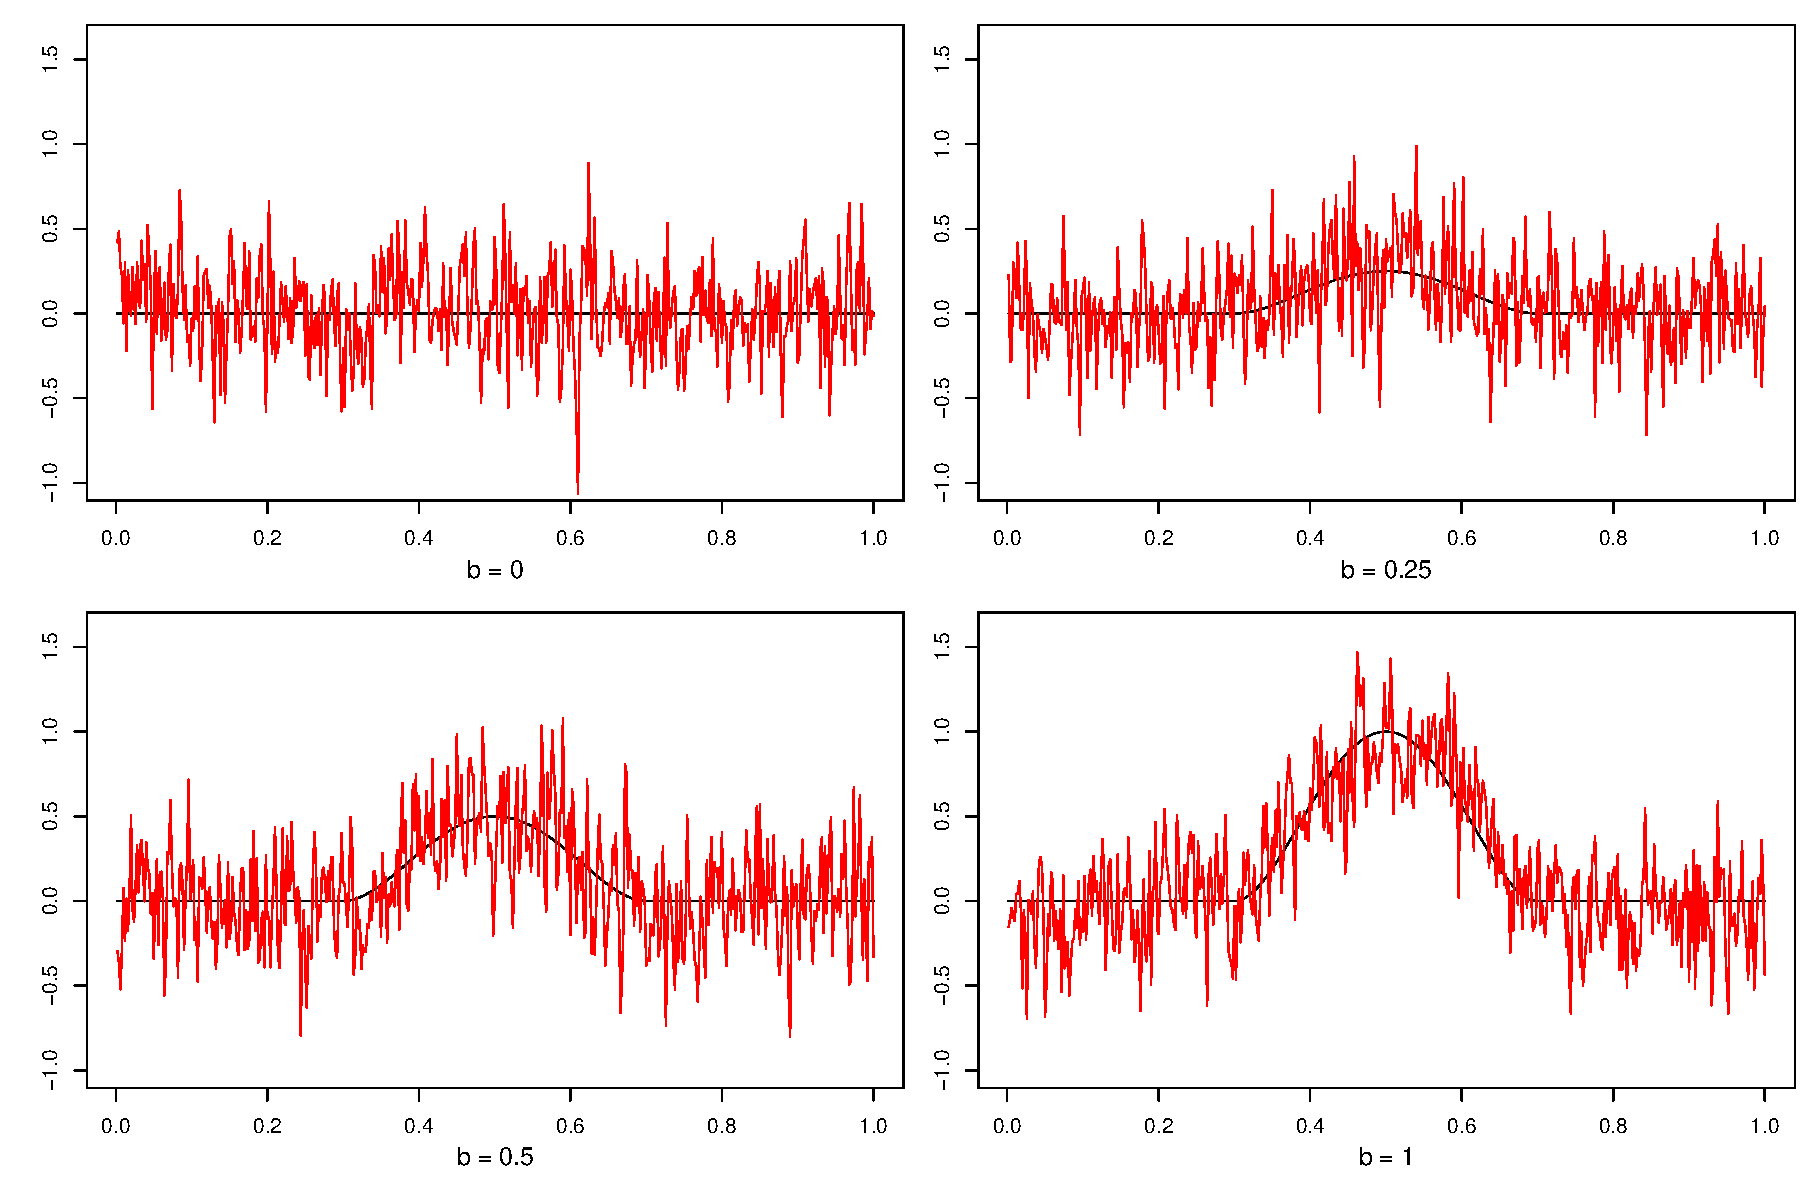
\includegraphics[width=\textwidth]{output/bump_function.pdf}
\caption{In black, the bump function $m_1$ is plotted for different heights of the bump: $b \in \{0, 0.25, 0.5, 1\}$ with $b=0$ corresponding to the null $H_0$. In red, we depict the time series $\{m_1(t/T) + \varepsilon_{1t}: 1 \le t \le T\}$ for one simulation run and $T=500$.}\label{fig:bump_function}

\end{figure}

\item We take the grid $\mathcal{G}_T$ to be the same as before: $\mathcal{G}_T = U_T \times H_T$, where $U_T = \big\{ u \in [0,1]: u = \textstyle{\frac{5t}{T}} \text{ for some } t \in \mathbb{N} \big\}$ and $H_T = \big\{ h \in \big[ \textstyle{\frac{\log T}{T}}, \textstyle{\frac{1}{4}} \big]:  h = \textstyle{\frac{5t - 3}{T}} \text{ for some } t \in \mathbb{N} \big\}$.

\item As before, in order to estimate the long-run error variance $\sigma^2$, we follow the procedure described in \citet{KhismatullinaVogt2020} with the following tuning parameters: $q = 25$ and $r = 10$.

\item As before, we calculate the Gaussian quantiles based on $5000$ samples. 

\item The number of simulation runs is $5000$. 

\end{itemize}

Figure \ref{fig:bump_function} illustrates that the described simulation setup is quite challenging already without covariates and fixed effects. The black lines in the plot show the bump function $m_1$ for different heights of the bump $b \in \{0, 0.25, 0.5, 1\}$, where the value $b=0$ corresponds to the null $H_0$ (as in this case, $m_1 = 0$ and we assume that $m_i = 0$ for all $i > 1$). The red line shows one realization of the time series $\{Y_{it}^*:1 \le t \le T \}$ for $T=500$, where 
\begin{equation}\label{eq:model-idealized}
Y_{it}^* = m_i\Big(\frac{t}{T}\Big) + \varepsilon_{it} 
\end{equation}
is the sum of the trend function and the noise term. Put differently, \eqref{eq:model-idealized} is an idealized version of our simulation design without covariates and fixed effects. The values $b=0.25,0.5,1$ correspond to three different alternatives. In particular, as the size of the bump $b$ gets larger, we move further and further away from the null. For the smallest value $b=0.25$, the bump function is extremely difficult to detect as the noise level is very high, or put differently, as the signal-to-noise ratio is very small (as can be seen from inspecting the upper right panel of Figure \ref{fig:bump_function}). For $b=0.5$ and $b=1$, the signal-to-noise ratio slowly gets bigger, making it less hard to detect the bump function. Nevertheless, even for $b=1$, there is substantial noise around the bump function, meaning that detection of the bump is still non-trivial. \\
The simulation results for the new more challenging design are reported in \textcolor{blue}{Section \ref{subsec:sim:main} of the Supplement}. 

\item We can assume that $m_i=0$ under $H_0$ without loss of generality for the following reason: First of all, note that given our normalization constraint $\int_0^1 m_i(u)du = 0$ for all $i$, the functions $m_i$ must be the same for all $i$ under $H_0$. Now consider the multiscale test statistic 
\[ \widehat{\Psi}_{n,T} = \max_{(u,h) \in \mathcal{G}_T, 1 \le i < j \le n} \Big\{ \Big| \frac{\widehat{\psi}_{ij,T}(u,h)}{(\widehat{\sigma}_i^2 + \widehat{\sigma}_j^2)^{1/2}} \Big| - \lambda(h) \Big\} \]
with
\[ \widehat{\psi}_{ij,T}(u,h) = \sum_{t=1}^T w_{t,T}(u,h) (\widehat{Y}_{it} - \widehat{Y}_{jt}). \]
Suppose we are under the null, that is, $m_i = m$ for all $i$ and an arbitrary trend function $m$. Since
\[ \widehat{Y}_{it} = m\Big(\frac{t}{T}\Big) + \varepsilon_{it} + (\boldsymbol{\beta}_i - \widehat{\boldsymbol{\beta}}_i)^\top \boldsymbol{X}_{it} + (\alpha_i - \widehat{\alpha}_i), \]
the function $m$ cancels out exactly (not only approximately!) in the difference $\widehat{Y}_{it} - \widehat{Y}_{jt}$. Moreover, it has a negligible effect on the estimator $\widehat{\boldsymbol{\beta}}_i$ as it essentially gets eliminated by the differencing operation. A similar point applies to the estimator $\widehat{\alpha}_i$ where $m$ shows up in the form of $\frac{1}{T} \sum m(t/T)$ which for large $T$ is very close to $\int_0^1 m(u) du = 0$. Hence, if we simulate data under the null with different functions $m$, we get (almost) identical values for the multiscale statistic $\widehat{\Psi}_{n,T}$. We can thus safely resort to setting $m=0$. 

\item %We have not considered any competing methods because there are not really any competitors out there. 
The main merit of our method is that we can perform inference \uline{uniformly over all pairs of time series $(i,j)$ and over all locations $u$ and bandwidths (or scales) $h$ in the grid $\mathcal{G}_T$}. Simple competitors (like the one you propose) are not uniform over the curves $(i,j)$ and bandwidths $h$ (as uniform confidence bands for nonparametric curves available in the literature depend on a specific choice of bandwidth). This implies that these simple competitors will be much too liberal. One could of course make a simple Bonferroni correction to fix this. However, as the underlying statistics will be strongly correlated across different $(i,j)$ and bandwidths $h$, this will result in extremely conservative procedures. We demonstrate this by comparing our approach with the SiZer method from \cite{Park2009} which is the closest competitor to our method (being a multiscale test which however is not uniform over scales $h$) Please see \textcolor{red}{the new Section ?? in the Supplement} for the details. 

\item In order to examine the performance of our method for larger $n$, we rerun our simulation exercises for $n \in \{25,50,100\}$ and $T$ as before, i.e., $T \in \{100,250,500\}$. We work with precisely the same simulation setup as specified in (i) except for the fact that we use a smaller grid $\mathcal{G}_T$ to decrease the computational burden a bit. Specifically, we take the grid 
\begin{align*}
\mathcal{G}_T = \big\{ (u,h) \subseteq [0,1]: & \ (u,h) = ((2s+1) h, h) \text{ for } s = 0,\ldots,\Big\lfloor \frac{h^ {-1}-1}{2} \Big\rfloor \\ & \ \text{and } h \in \mathcal{H}_T \big\},  
\end{align*}
that is, we work with a dyadic scheme (as in Wavelet analysis) with scales in the set 
\[ \mathcal{H}_T = \big\{ h = 2^k h_{\min} \text{ for } k=0,\ldots,K \big\}, \]  
where $h_{\min} = \frac{\lceil \log T \rceil}{T}$ and $K$ is such that $2^K h_{\min} \le \frac{1}{4}$, i.e.,
\[ K \le \Big\lfloor \log\Big(\frac{T}{4 \lceil \log T \rceil }\Big) \Big\rfloor \frac{1}{\log(2)}. \]
Overall, the simulation results show that the method performs well for larger $n$. Please see \textcolor{red}{Section ?? in the Supplement} for the details. 

\end{enumerate} 


\item \textit{Similarly, there are many related clustering methods, including (Bayesian and non-Bayesian) methods for clustering functional data. The proposed approach is reasonable, yet should be placed in a broader context and evaluated against appropriate competitors.}
  
We compare our clustering approach with the following benchmark: 
\begin{itemize}[leftmargin=0.45cm,itemsep=0pt,topsep=0pt]
\item Estimate the trends $m_i$ by a local linear estimator $\hat{m}_i(\cdot,h)$ with bandwidth $h$ (chosen adhoc).
\item Compute a simple distance measure $d_{ij}$ between $\hat{m}_i$ and $\hat{m}_j$, e.g.
\[ d_{ij} = \int_0^1 (\hat{m}_i(w) - \hat{m}_j(w))^2 dw. \]
\item Construct the following dissimilarity measure from these distances:
\[ \hat{\Delta}(S,S') = \max_{i \in S,j \in S'} d_{ij}. \]
\item Run a HAC (agglomerative hierarchical clustering) algorithm with the computed dissimilarities. 
\end{itemize}
This procedure is a very simple and natural benchmark, our approach being a refinement of it. In particular: our approach replaces the simple distance measure $d_{ij}$ by a more advanced multiscale distance measure and provides a way to estimate the number of clusters, which is not part of the simple benchmark procedure. A comparison study is presented in \textcolor{red}{Section ?? of the Supplement}. Most importantly, it shows that our method provides robust results whereas the benchmark depends very strongly on the choice of bandwidth.  

    
\item \textit{A related Bayesian strategy is to use simultaneous band scores (simBaS) to assess whether a function differs from zero. This could be applied pairwise to the differences between functions to establish a Bayesian competitor to the proposed approach, and simply requires posterior draws from an analogous Bayesian model.}

We mention simBaS as a possible competitor in \textcolor{red}{Section ?? of the Supplement} where we compare with the SiZer method from \cite{Park2009} (as discussed in our reply to your comment 2(iii)). In view of the many other extensions and robustness checks carried out, we have decided not to run simulations on any other competitors besides SiZer. We hope you are fine with this. 

  
\item \textit{The application includes numerous tuning parameters (including kernels, intervals, etc.). Are the results robust to these choices? Further details are needed.}
  
In the revision, we have carried out a number of robustness checks on the choice of tuning parameters. Please see \textcolor{red}{the new Section ?? of the Supplementary Material} for the details. In addition, please also see our reply to comment 4 of the associate editor. \\
The main tuning parameter of our methods is the grid $\mathcal{G}_T$. As a robustness check, we have run the simulation exercises from Section ?? for three different grids: the grid defined in the description of the simulation setup above as well as a sparser and a denser grid (\textcolor{red}{see p.?? in the Supplementary Material} for a precise definition). All three grids are sufficiently rich in the sense of incorporating a wide range of bandwidths (from very small to very large ones) and many time points that are scattered rather densely over the unit interval. The simulation results are very similar across the different grid specifications, indicating that our methods are insensitive to the precise choice of grid (as long as it is sufficiently rich). \\
Further tuning parameters of our methods are (i) the number of bootstrap samples $L$ to compute the Gaussian quantile, (ii) the kernel $K$ and (iii) tuning parameters to estimate the long-run error variance $\sigma^2$. 
The number of bootstrap samples $L$ is set to $5000$ throughout the simulation study. As a robustness check, we have rerun everything with $L=1000$. As expected, the results are essentially identical. We have added a short remark on this to \textcolor{red}{p.?? of the Supplement}, but we have not reported the results. However, we are happy to do so if you think this is needed.
As suggested by classical nonparametric theory, the Epanechnikov kernel (which is used throughout the paper) has good properties and the choice of kernel $K$ is of minor importance, in particular, much less important than the choice of bandwidth. We have thus decided not to run any robustness checks on the choice of kernel. 
Finally, our procedure can be combined with any method off-the-shelf for long-run error variance estimation. In the simulations and the empirical applications of the paper, we use the procedure from \cite{KhismatullinaVogt2020}, where extensive robustness checks w.r.t.\ to the choice of tuning parameters have been performed. We have thus not included further robustness checks on these secondary tuning parameters in the paper.   
\textcolor{red}{[Re-run everything with true error variance?]}

  
\item \textit{The multiscale tests are designed to control the FWER. Why is that the right criterion for the types of applications in mind (compared to e.g., FDR)? Given that other reasonable choices exist, additional motivation for this objective is warranted.}

Let $\alpha$ be a given value, say $\alpha = 0.05$. 
\begin{enumerate}[label=(\roman*),leftmargin=0.75cm,topsep=0pt]
\item Controlling the FWER allows us to make the following type of confidence statements: We can claim with statistical confidence at least $1-\alpha$ (formally, with asymptotic probability at least $1-\alpha$), that the differences between the trends detected by our test method reflect true differences in the underlying curves. 
\item Controlling the FDR would only allow us to make statements of the following form: We can claim that (on average) $100(1-\alpha) \%$ of the differences detected by our test correspond to true differences.
\end{enumerate}
We think that in economic and financial applications, one is usually interested in statements of the form (i) rather than (ii). Take a financial example where one aims to compare volatility trends of different stocks. Practitioners want to make interpretations based on the differences found by the test. For instance, they would like to connect them to certain market events. For this, they want to be rather confident that the detected differences are worth interpreting (i.e.\ are not spurious but correspond to real differences). It is not enough to be confident that (on average) a certain percentage of the detected differences are worth interpreting. Hence, in our opinion, confidence statements of the form (i) are more apt than statements of the form (ii) in this context. \\
\textcolor{blue}{We have added these remarks on FWER vs.\ FDR control to Section 3.3 of the paper. See in particular Remark 3.2 therein.}


\item \textit{I'm wondering if there might be some clarification about the independence of $\varepsilon_{it}$ across series $i$. In particular, suppose the intercepts $\alpha_i$ were instead considered random, like in mixed modeling (or Bayesian inference). Then marginally, the ``new'' errors ($\alpha_i + \varepsilon_{it}$) would be dependent across series $i$. Similar reasoning might apply to the covariates. From this perspective, the class of models might be considered more general.}

First of all, please note the terms $\alpha_i$ are not restricted to be deterministic. They can be either deterministic or random, we do not impose any distributional assumptions on them, and they can be correlated with the covariates $\boldsymbol{X}_{it}$ in an arbitrary way. Following the panel data literature in economics, we refer to them as fixed effects (which one may find extremely misleading beacuse ``fixed'' sounds like they are restricted to be deterministic). In the revision (\textcolor{blue}{see p.??}), we have added some additional remarks on the terms $\alpha_i$ to avoid any confusion. \\
Following your suggestion, we point out in the revised paper (\textcolor{blue}{see p.??}) that we allow for dependencies in the error terms ($\alpha_i + \varepsilon_{it}$) across time series $i$ via the inclusion of the fixed effects $\alpha_i$.   
  
  
\item \textit{It is claimed on p.6 that the mean function integrating to zero is ``required'' for identification of the intercept. I think this is a sufficient, not necessary, condition, since others might suffice.} 

We agree that the wording is a bit misleading. We have thus changed it. We use the constraint $\int_0^1 m_i(u) du = 0$ for identification as it yields a convenient normalization. However, it is of course possible to work with other constraints instead. 

  
\end{enumerate}



\subsection*{Reply to referee 2}


Thank you very much for the careful reading of our manuscript and the interesting suggestions. We have addressed all your comments in the revision. Please see our replies to them below.
\begin{enumerate}[label=\arabic*.,leftmargin=0.6cm]

  
\item \textit{Although you correctly cite Khismatullina and Vogt (2020, 2021) on which quite a bit of this new work seems to be based can you please summarize more in particular about the test proposed in Khismatullina and Vogt (2021, Journal of Econometrics), and explain where and how your proofs differ from that (e.g.\ by the complexity in needing to treat the covariates).}

\cite{KhismatullinaVogt2021} consider the following setting: Let $Y_{it}$ be the number of new corona infections on day $t$ in country $i$ and suppose we observe a data sample $\{Y_{it}: 1 \le t \le T \}$ for $n$ different countries $i$. A simple way to model the count data $Y_{it}$ is by means of a Poisson distribution. In particular, we may assume that $Y_{it}$ is Poisson distributed with time-varying intensity parameter $\lambda_i(t/T)$, that is, $Y_{it} \sim \mathcal{P}_{\lambda_i(t/T)}$. This model can be formulated as
\begin{equation}\label{eq:poisson-model}
Y_{it} = \lambda_i\Big(\frac{t}{T}\Big) + u_{it} \quad \text{with} \quad u_{it} = \sqrt{ \lambda_i\Big(\frac{t}{T}\Big) } \eta_{it}, 
\end{equation}
where $\eta_{it}$ is a noise term with zero mean and unit variance. \eqref{eq:poisson-model} is a nonparametric trend model, where the trend and the (time-varying) variance of the error term $u_{it}$ are given by the intensity function $\lambda_i$. For applications, however, the assumption that the trend and the error variance are exactly the same is usually too restrictive. \cite{KhismatullinaVogt2021} thus propose the quasi-Poisson model 
\begin{equation}\label{eq:quasi-poisson-model}
Y_{it} = \lambda_i\Big(\frac{t}{T}\Big) + u_{it} \quad \text{with} \quad u_{it} = \sigma \sqrt{ \lambda_i\Big(\frac{t}{T}\Big) } \eta_{it}, 
\end{equation}
which extends \eqref{eq:poisson-model} by including the scaling factor $\sigma$. This allows the variance to be a multiple of the trend function. This model is not nested in our framework as the error terms $u_{it}$ have a (very particular) nonstationary structure. Nevertheless, it is much simpler in most other respects: The noise terms $\eta_{it}$ are assumed to be i.i.d.\ both across $i$ and $t$, implying that there are no dependence structures at all in the model. Moreover, there are no covariates and fixed effects included. \\
The multiscale test in \cite{KhismatullinaVogt2021} is similar in spirit to the one analyzed in the current paper. However, their theoretical analysis is completely different. In particular, their proofs build on high-dimensional CLTs for hyperrectangles developed in \cite{Chernozhukov2017}, while our proofs rely on results from strong approximation theory. Hence, even without the inclusion of covariates and fixed effects, our proof strategy would be completely different. The issue is that the arguments in \cite{KhismatullinaVogt2021} rely heavily on the i.i.d.\ structure of the data and can thus not be carried over to the current model setting as far as we can see. \\
We haved added a condensed version of the above discussion to the revision (\textcolor{blue}{see p.?? in the introduction} and \textcolor{blue}{Remark 4.3 in Section 4}). 


\item \textit{As your results are of asymptotic nature, it would be good to discuss limitations -- even give an example where the procedure would cease to work.}  

As we discuss in response to your comment 4 below, our method will in general have poor small sample performance when the error and covariate processes are very persistent. For example, when the error process is autoregressive of order $1$ with parameter close to the unit circle (say $0.95$ or $0.99$), the procedure will break down in small samples (even though our asymptotic theory allows for an AR(1) error process with parameter $0.95$ or $0.99$). We discuss this limitation \textcolor{red}{on p.?? of the revision [It may be best to discuss this to the simulations and thus to motivate that we look at AR processes with coefficients $0.25$ rather than $0.95$]}. Please also see our answer to your comment 4 for more details.
  

\item \textit{Moreover, can you at least sketch out if by something like a Bootstrap procedure (cf.\ Zhang et al, 2012) more of the ``asymptotic flavour'' of your test/cluster procedure could be remedied?}

To be honest, it is not so clear to us how to set up a good bootstrap procedure. In what follows, we sketch some ideas and discuss the implied issues. To make things easier, consider the simplified model 
\[ Y_{it} = m_i\Big(\frac{t}{T}\Big) + \varepsilon_{it} \]
without covariates and fixed effects and assume that the errors $\varepsilon_{it}$ are i.i.d.\ both across $i$ and $t$. In this simplified model, one may set up a multiplier or wild bootstrap by resampling the statistics
\[ \widehat{\psi}_{ij,T}(u,h) = \sum_{t=1}^T w_{t,T}(u,h) (\widehat{Y}_{it} - \widehat{Y}_{jt}), \]
which are the main building block of our multiscale statistic $\widehat{\Psi}_{n,T}$. In particular, one may proceed as follows: Draw a large number $L$ of samples $S^{(\ell)} := \{\xi_{it}^{(\ell)}: 1 \le t \le T, 1 \le i \le n \}$ for $\ell=1,\ldots,L$, where $\xi_{it}^{(\ell)}$ are i.i.d.\ standard normal random variables. (Note that other distributions are possible here.) Then compute the resampled statistics  
\[ \widehat{\psi}_{ij,T}^{(\ell)}(u,h) = \sum_{t=1}^T w_{t,T}(u,h) (\widehat{Y}_{it} \xi_{it}^{(\ell)} - \widehat{Y}_{jt} \xi_{jt}^{(\ell)}) \]
and the corresponding multiscale statistic $\widehat{\Psi}_{n,T}^{(\ell)}$ for $\ell=1,\ldots,L$. Finally, take the empirical $(1-\alpha)$-quantile of the bootstrap sample $\{ \widehat{\Psi}_{n,T}^{(\ell)}:  \ell=1,\ldots,L \}$ as the critical value of the test. \\
We guess that this bootstrap approach should work. However, it will be conservative because under the alternative, the variance level of $\widehat{Y}_{it} \xi_{it}^{(\ell)}$ is in general higher than the target $\text{Var}(\varepsilon_{it})$. One could fix this by subtracting an estimator of $m_i(t/T)$ from $\widehat{Y}_{it}$ before multiplying with $\xi_{it}^{(\ell)}$. However, to estimate $m_i(t/T)$ nonparametrically, we'd need to introduce an additional bandwidth parameter (for each $i$), which goes somewhat against the philosophy of our multiscale approach). Moreover, when the errors $\varepsilon_{it}$ are not independent across $t$, one would have to correct the approach to take into account the time series correlation in the errors. Apart from these issues, it is not clear whether such a wild bootstrap approach has better theoretical properties than our simulation approach. We have thus decided not to include specific suggestions for bootstrap procedures in the paper. However, we fully agree with you that it is an interesting issue how to set up a good bootstrap in our case. We thus briefly mention this as an open question \textcolor{blue}{in the new conclusion section (Section 8)}. 


\item \textit{I am having a slight (finite sample) identification concern with (not only your) model(s) mixing deterministic (nonparametric) trends with covariate (and also error) structure which is allowed to be positively serially dependent, e.g.\ autoregressive (as in your examples): I think that for ``any'' fixed sample size it might always occur that the trajectory of a stochastic trend, an autoregressive process with roots relatively close to the unit circle, say, cannot be distinguished from the deterministic trend. Wouldn't that be potentially a problem for your (and any related) test procedure? As a follow-up on this, wouldn't you need (or to say it differently, wouldn't it be perhaps beneficial to add) some extra conditions on the nature of your covariates (and potentially also your errors $\varepsilon$?) to avoid this problem?}

We fully understand the issue you point out. One may model a time series trend by a deterministic function plus noise (as we do), by a very persistent stationary process (such as an AR process with roots close to the unit circle) or by a nonstationary process (such as a unit root process). In small samples, it is essentially impossible to reliably tell how the trend is generated (whether it is deterministic or stochastic, and if stochastic, whether it is produced by a stationary or a nonstationary process). Asymptotically, it is of course possible to discern these cases by a formal statistical test. However, such a test will have power only for quite large sample sizes and will thus be rather useless in smaller samples. \\
What does this mean for our procedure? To obtain good performance in small samples, we require that the error (and covariate) process in our model does not produce strong stochastic trends. For our asymptotic theory to work, it is sufficient to assume that the error (and covariate) process is stationary and short-range dependent. However, this includes very persistent processes like AR processes with roots close to the unit circle. Hence, the conditions for our asymptotic theory are not sufficient to guarantee good performance in small samples. Loosely speaking, to guarantee good small sample performance, we require the persistence of the error (and covariate) process to be sufficiently mild. In our simulations where $T=\{100,250,500\}$, we can for example deal well with AR(1) errors with autoregressive coefficient $0.25$ or $0.5$. However, if we considered an AR(1) error process with $0.95$, the procedure would clearly break down. \\
We discuss these points \textcolor{red}{on p.?? in the revision [It may be best to discuss this to the simulations and thus to motivate that we look at AR processes with coefficients $0.25$ rather than $0.95$]}.

%\begin{enumerate}[label=(\roman*),leftmargin=0.75cm,topsep=0pt]
%\item We totally agree with you. It is extremely difficult to distinguish a deterministic from a stochastic trend in a given data sample of fixed size. Let us consider the following simple model to illustrate this: Suppose we observe (only) one time series $\{Y_t: 1 \le t \le T\}$ which follows the trend-plus-noise model
%\[ Y_t = m\Big(\frac{t}{T}\Big) + \varepsilon_t, \]
%where $m$ is the trend function and $\{\varepsilon_t\}$ is a very persistent (zero-mean) error process, say an AR(1) process with parameter $0.99$. Even though stationary, this process produces trend-like time series paths. In small samples, it is virtually impossible to distinguish the deterministic trend $m$ from the trend-like patterns produced by the AR error. Put differently, in small samples, it is essentially impossible to reliably estimate the trend function $m$ or make inference on it -- no matter which statistical procedure is used.
%\item %What does that mean for our procedure (as well as for any other procedure for trend detection)? To obtain good small sample performance, one requires that the error process is not too persistent. For example, if we consider time series of length T $T=100, 250, 500$ and an AR(1) error as in our simulations, the AR coefficient should not be too close to $1$.
%From an asymptotic point of view, it is enough to assume that the error process is stationary and short-range dependent (which e.g.\ includes the AR(1) process with parameter $0.99$) from above. However, to obtain good small sample performance, one requires that the error process is not too persistent. So if we consider time series of length T $T=100, 250, 500$ and an AR(1) error as in our simulations, the AR coefficient should not be too close to $1$. (The same points apply of course to the covariate processes.)
%\end{enumerate}
%We discuss points (i) and (ii) in the revision on p.??. 


\item \textit{What about a naive competitor that is just based on the second derivative (= change of the slope parameters) rather than the distance based on the curves and the first derivative (as in your local linear estimator)? I believe that this could also work rather well on your economic example data in Figures 3--6? Maybe you can ``benchmark'' your procedure against such a simple competitor (as such a comparison is somewhat missing explicitly -- although you orally compare sometimes with Zhang et al (2012)).}

\textcolor{red}{TO DO. Not sure what is meant here!} \textcolor{orange}{Any ideas, Marina?}


\item \textit{Can your proposed test procedure be considered somehow to be equivalent to constructing a uniform confidence region where you would need to control if two (or more curves) are within the same tube (not just pointwise)? If so, it would be perhaps interesting to explain the link, and why for your test procedure it is sufficient/adequate to control the ``familywise'' error (does this correspond to what one does for a ``uniform'' region?).}

One can make the following connection to uniform confidence regions: 
\begin{itemize}[leftmargin=0.45cm,itemsep=0pt,topsep=0pt]

\item The main building block of our test statistic is the local average
\[ \widehat{\psi}_{ij,T}(u,h) = \sum_{t=1}^T w_{t,T}(u,h) (\widehat{Y}_{it} - \widehat{Y}_{jt}). \]
Since the weights $w_{t,T}(u,h)$ are rescaled versions of the kernel weights of a standard local linear kernel estimator \citep{FanGijbels1996}, $\widehat{\psi}_{ij,T}(u,h)$ is nothing else than a rescaled difference between local linear estimators of $m_i(u)$ and $m_j(u)$ with bandwidth $h$. 

\item Now consider 
\[ \psi_{ij,T}(u,h) = \sum_{t=1}^T w_{t,T}(u,h) \Big(m_i\Big(\frac{t}{T}\Big) - m_j\Big(\frac{t}{T}\Big)\Big), \]
which is a weighted local average of the difference between the functions $m_i$ and $m_j$ on the interval $[u-h,u+h]$. Our theoretical results imply that with asymptotic probability $1-\alpha$, 
\[ \big| \widehat{\psi}_{ij,T}(u,h) - \psi_{ij,T}(u,h) \big| \le c_{n,T}(\alpha,h) \]
for all $(u,h) \in \mathcal{G}_T$ and $1 \le i < j \le n$, where $c_{n,T}(\alpha,h) := (\widehat{\sigma}_i^2 + \widehat{\sigma}_j^2)^{1/2} (q_{n,T}(\alpha) + \lambda(h))$ with $q_{n,T}(\alpha)$ the global critical value of our multiscale test and $\lambda(h)$ defined in Section 3.2 of the paper. 

\item We can interpret the result from the previous bullet point as a uniform confidence band for the parameter $\psi_{ij,T}(u,h)$ (uniform over all $(u,h)$ and $i < j$ under consideration). In particular, we get that with asymptotic probability $1-\alpha$, $\psi_{ij,T}(u,h)$ lies in the confidence interval
\begin{align*}
\text{CI}_{ij,T}(u,h) := \Big[ & \widehat{m}_{i}(u,h) - \widehat{m}_{j}(u,h) - c_{n,T}(\alpha,h), \\ & \qquad \widehat{m}_{i}(u,h) - \widehat{m}_{j}(u,h) + c_{n,T}(\alpha,h) \Big].
\end{align*}  

\item Our test can now be equivalently formulated as follows: We reject the local null hypothesis
\[ H_0^{[i,j]}(u,h): m_i \text{ and } m_j \text{ are the same on the interval } \mathcal{I}_{u,h} = [u-h,u+h] \]
if the uniform confidence band $\text{CI}_{ij,T}(u,h)$ does not include $0$. 

\end{itemize} 
We have added a condensed version of the above discussion to the revision. Please see \textcolor{blue}{the new Remark 3.1 therein}. 


\item \textit{How in all of this does the number of curves (larger than two) play a role, in practice, for correctly calibrating your test (as least asymptotically as possible)? On the other hand, do your results reflect the fact that obviously they depend on the number of time series (or rather the number of series where trends are different, a number that you would have access to in an oracle situation)?}

The critical value $q_{n,T}(\alpha)$ of the multiscale test is defined as the $(1-\alpha)$-quantile of the Gaussian statistic 
\begin{align}\label{eq:Phi}
\Phi_{n,T} = \max_{1 \le i < j \le n}\max_{(u, h) \in \mathcal{G}_T} \Big\{ \bigg|\frac{\phi_{ij, T}(u, h)}{(\sigma_i^2 + \sigma_j^2)^{1/2}}\bigg| - \lambda(h) \Big\},
\end{align}
where
\begin{align*}
\phi_{ij, T}(u, h) = \sum\limits_{t=1}^T w_{t,T}(u, h) \, \big\{ \sigma_i (Z_{it} - \bar{Z}_i) - \sigma_j (Z_{jt} - \bar{Z}_j) \big\},
\end{align*}
with $Z_{it}$ being independent standard normal random variables for $1 \le t \le T$ and $1 \le i \le n$ and $\bar{Z}_i = \bar{Z}_{i,T} := T^{-1} \sum_{t=1}^T Z_{it}$. As one can see, the statistic $\Phi_{n,T}$ depends on both the number of time series $n$ and the time series length $T$. This implies that its $(1-\alpha)$-quantile and thus the critical value of the multiscale test depends on both $n$ and $T$. Hence, the calibration of the test (or put differently, the choice of the critical value) is very ``un-asymptotic'' in the sense of reflecting the size of $n$ and $T$. 


\item \textit{Here is a small series of remarks towards needing to choose $(u, h)$ -- an example for a practical choice is given in Section 7, only (a bit late): Your localised multiscale method requires to discretize the continuous $(u, h)$. I am wondering if the way to do this plays a role for the properties of the resulting practical procedure. Can you please also compare with wavelet-based multiscale methods which are based somehow on a ``built-in'' way of choosing the location-scale parameters $(u, h)$?}  

In the revision, we give an example of such a practical choice much earlier (\textcolor{blue}{see the last few sentences in Section 3.2}). \\
Our methods take into account all points $(u,h)$ in the discrete grid $\mathcal{G}_T$ (which is finite but grows with sample size). As one can see from equation \eqref{eq:Phi}, the Gaussian statistic depends on the grid $\mathcal{G}_T$. Hence, the test is calibrated differently depending on the grid. In that sense, the test adapts to the choice of grid: if the grid is quite sparse, the critical value will tend to be smaller, if it is quite fine, it will be larger. One can show formally (at least for a very simplified version of our multiscale test; also see the results in \cite{DuembgenSpokoiny2001}) that the critical value becomes stable if we make the grid finer and finer. This means that the exact choice of the grid (i.e.\ the exact way of discretizing) should play a negligible role as long as the grid is not chosen too sparse. In the revision, we support this claim by simulation evidence. Please see the new robustness checks in \textcolor{red}{Section ?? of the Supplement} where we run our methods with different grids. We in particular include a dyadic grid which is (to use your words) the ``built-in'' way of choosing the location-scale parameters $(u, h)$ in wavelet analysis. Please also see our reply to comment 5 of referee 1. 


\item \textit{page 12, around equation (3.6): it took me a moment to understand that you are talking about the standard local linear estimator (of Fan and Gijbels) here, you might want to make this clearer.}

We have made this clearer now. Please see \textcolor{blue}{the beginning of Section 3.2 in the revision} where we write: ``Note that the weights $w_{t,T}(u,h)$ are rescaled versions of the kernel weights of a standard local linear estimator \citep{FanGijbels1996}. Hence, the statistic $\widehat{\psi}_{ij, T}(u, h)$ is nothing else than a rescaled difference between local linear estimators of $m_i(u)$ and $m_j(u)$ with bandwidth $h$.''    


\item \textit{I understand the heuristics behind using the Gaussian version (3.12) of the test statistics in the ``idealised'' situation but what about the ``non-idealised'' situation of unknown variances $\sigma^ 2$ and unknown parameters $\beta$? Is the Gaussian-based MC simulation method still valid when you need to estimate those parameters?}  

Yes, the Gaussian-based MC simulation method is still valid when $\sigma^2$ and $\boldsymbol{\beta}_i$ are estimated. In particular, as stated in Proposition 4.3, our multiscale test has (asymptotically) the correct size $(1-\alpha)$ under the null if we take the $(1-\alpha)$-quantile of the Gaussian statistic (3.12) to be the critical value of the test. In the proof of Theorem 4.1 (which underlies Proposition 4.3), it is formally shown that the effect of estimating $\sigma^2$ and $\boldsymbol{\beta}_i$ is negligible (see Step 1 of the proof for $\sigma^2$ and Step 4 of the proof for $\boldsymbol{\beta}_i$).
  

\item \textit{Again about the choice of $(u, h)$: what happens with expressions (such as in equation (4.1)) which depend on $\max_{(u,h)}$ in practice where you have to discretize this $(u, h)$? I do not think that a maximum over a continuous location-scale parameter can be treated the same way as one over a discrete one? Does the choice of the grid $\mathcal{G}_T$ influence the results here, don't you need some (additional) conditions on the grid (its spacing etc)? This refers, e.g.\ to the simulation section 6, page 24 where -- in passing -- you might want to change the strange wording there where you say ``for some t in N'' and rather detail the specification of the grid in $t$ here as you do later in Section 7.}  

All maxima in the paper are taken over a finite number of points. For example, the maximum in equation (4.1) is taken over all pairs $(i,j)$ with $1 \le i < j \le n$ and over all $(u,h)$ in the finite grid $\mathcal{G}_T$. Hence, we consider a finite grid of points $(u,h)$ in both theory and practice. (Note that in our theoretical considerations, we let the grid size grow with the sample size.) \\
Please see our reply to your comment 8 on how the choice of grid $\mathcal{G}_T$ influences our methods. \\
We do not need extra conditions on the grid $\mathcal{G}_T$ because the family of hypotheses $\{H_0^{[ij]}(u,h): 1 \le i < j \le n, (u,h) \in \mathcal{G}_T \}$ that we test depends on the chosen grid $\mathcal{G}_T$. Hence, if we have a small/large grid, we test a small/large number of hypotheses. As an extreme (admittedly a boring one, but it nevertheless helps to make the point), if the grid $\mathcal{G}_T$ only contains a single point, say $(u,h) = (0.5, 0.1)$, then we can only make confidence statements about the trend functions $m_i$ on the interval $[0.5-0.1,0.5+0.1]$. \\
Finally, as you suggest, we have changed the wording on p.24 in the previous version of the paper (\textcolor{red}{see p.?? in the revision}). 


\item \textit{Section 7, page 41, lines 45-50: can you develop this conjecture a bit?}

We guess you mean the conjecture on ``Section 7, page 31, lines 45-50''. Let us briefly repeat this conjecture: Contrary to \cite{Knoll2017}, our test finds significant differences in the trending behaviour of the observed time series, specifically, between the time trends of Belgium and Denmark and of Belgium and the USA (see Figures 5 and 6 in the paper, respectively). We conjecture that this discrepancy in the results is ``due to the fact that the method used in \cite{Knoll2017} does not account for effects of other factors such as GDP or population growth, while our test allows to include various determinants of the average house prices in model (7.1)''. We in particular believe that the rate of population growth is the main factor that causes the discrepancy in the results. The influence of this factor on house prices greatly varies across countries. Specifically, the estimated regression coefficient of the population growth rate for Belgium (BEL), Denmark (DNK) and the USA is $\widehat{\beta}_{\text{BEL}, 2} = 3.45$, $\widehat{\beta}_{\text{DNK}, 2} = 0.19$ and $\widehat{\beta}_{\text{USA}, 2} = 0.80$, respectively. \\
To substantiate our conjecture, we have repeated the analysis from the current Section 6 (Section 7 previously) with one distinction: we do not include the population growth rate as a regressor in the model.
%For the sake of brevity, we focus on the two comparisons Belgium vs.\ Denmark and Belgium vs.\ USA.
As conjectured, our test does not find any significant differences between Belgium and Denmark and between Belgium and the USA in this case (see Figures \ref{fig:hp:Belgium:Denmark} and \ref{fig:hp:Belgium:USA} above), which is in line with the findings presented in \cite{Knoll2017}. \\
We have added a few more sentences on our conjecture \textcolor{blue}{to Section 6 on p.27-28}. 

\begin{figure}[t!]
\begin{minipage}[t]{0.48\textwidth}
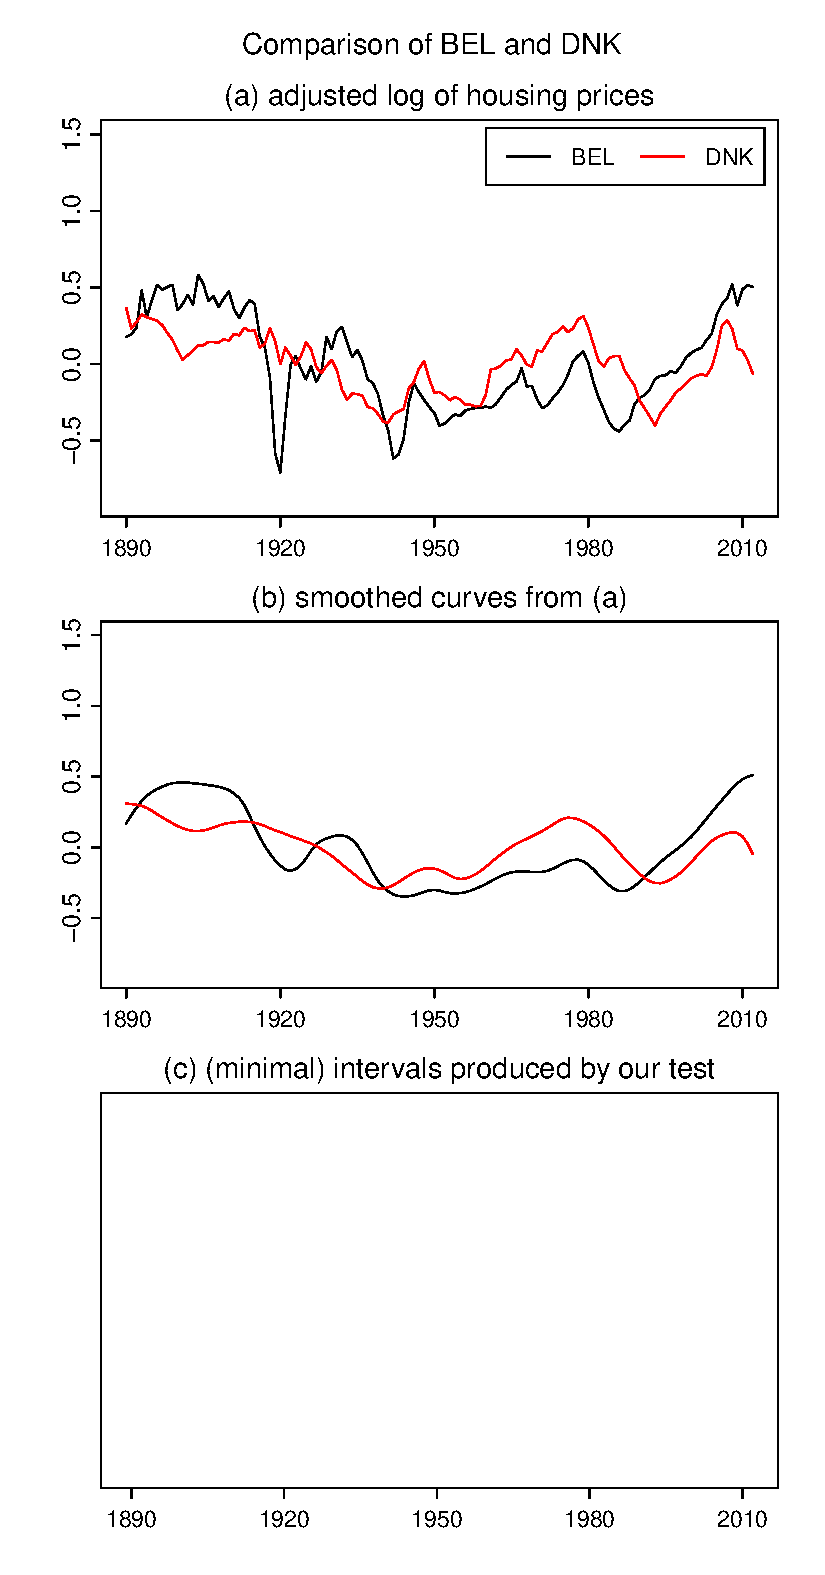
\includegraphics[width=\textwidth]{output/BEL_vs_DNK}
\caption{Test results for the comparison of the house prices in Belgium and Denmark not accounting for population growth.}\label{fig:hp:Belgium:Denmark}
\end{minipage}
\hspace{0.1cm}
\begin{minipage}[t]{0.48\textwidth}
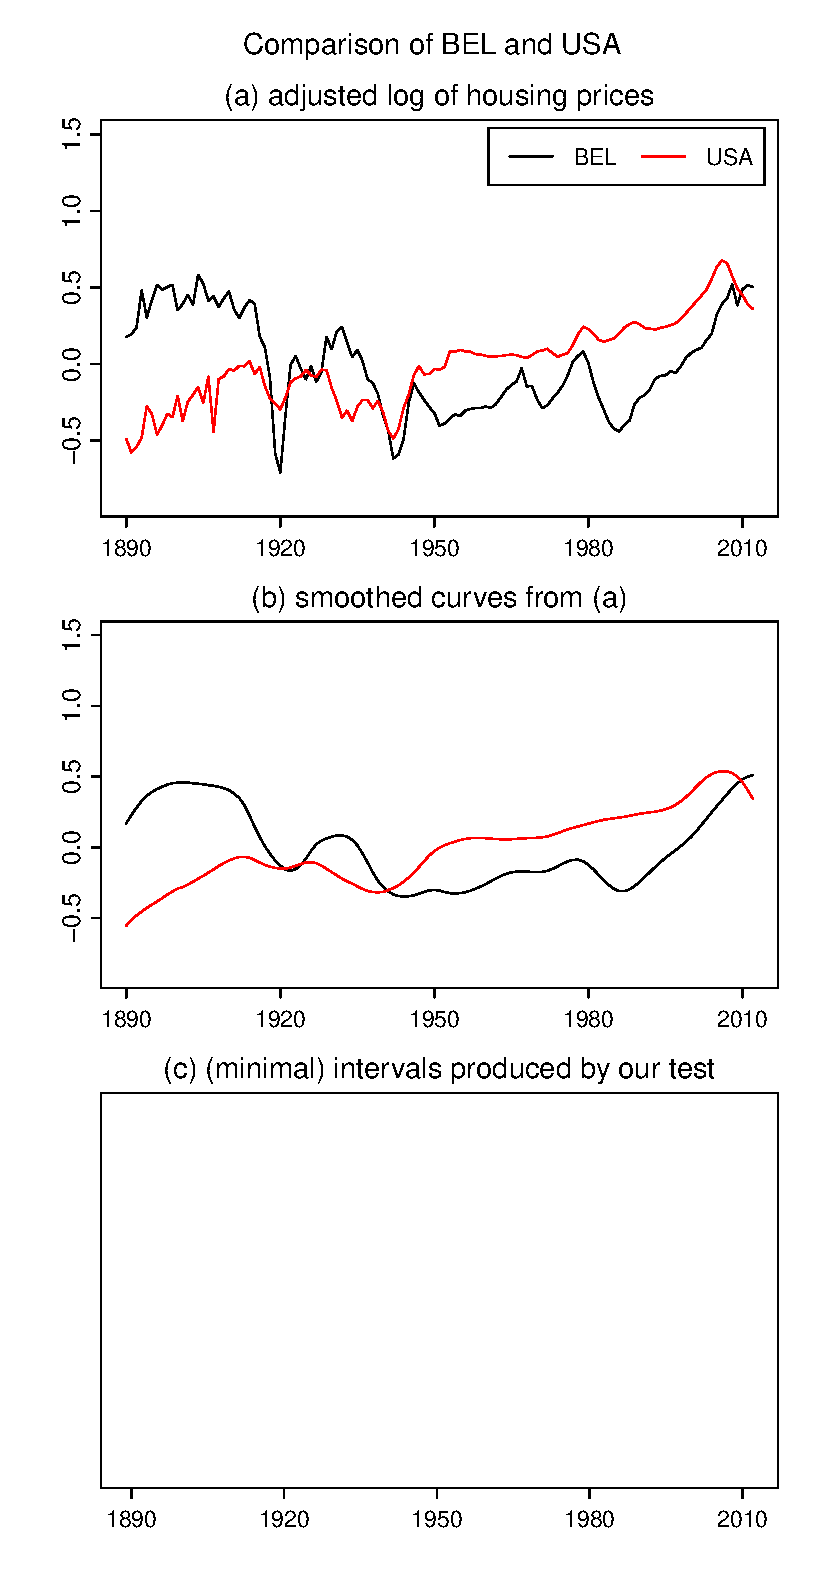
\includegraphics[width=\textwidth]{output/BEL_vs_USA}
\caption{Test results for the comparison of the house prices in Belgium and the USA not accounting for population growth.}\label{fig:hp:Belgium:USA}
\end{minipage}
\caption*{Note: In each figure, panel (a) shows the two augmented time series of the house prices, panel (b) presents smoothed versions of the augmented time series, and panel (c) depicts the set of intervals $\mathcal{S}^{[i, j]}(\alpha)$, which is empty in the present case.}
\end{figure}

%We believe that the main factor that caused the discrepancy in the results is the rate of the population growth. Even though Belgium, Denmark and the USA have maintained a relatively stable population growth rate, with minor fluctuations over the whole time period under consideration, the influence of this factor greatly varies across the countries. Specifically, we estimate $\beta_{\text{BEL}, 2} = 3.45$, $\beta_{\text{DNK}, 2} = 0.19$ and $\beta_{\text{USA}, 2} = 0.80$. The variation in the effect that population growth has on housing prices may be attributed to the disparities in housing supply elasticity, land availability, and urbanization rates. Furthermore, economic conditions, policy frameworks, and investment patterns also influence this relationship. Hence, accounting for the effect of the population growth on the housing prices may lead to significant changes of the adjusted time series (compare panels (a) in Figure \ref{fig:hp:Belgium:Denmark} and \ref{fig:hp:Belgium:USA} where assume that there are only three determinants of the house prices, real GDP, long-term interest rate and inflation, and panels (a) in Figures 5 and 6 in the main body of the paper).

%However, we believe that the population growth is one of the key determinants of the real house prices, and thus, needs to be accounted for by including it in the model. Hence, we have decided to add this robustness check to the Appendix rather than to the main body of the paper.


\item \textit{You might want to add a Conclusion Section which could both serve to recall the difficulties encountered in treating the more general situation of more than two curves and the presence of
covariates, and also discuss some of the aforementioned points on Bootstrap alternatives or on potential competitors.}  

As suggested, we have added a conclusion section (\textcolor{blue}{see the new Section 7}) where we discuss these points. 


\item \textit{Develop more to which extent the second data application (in the Supplement) brings insights beyond the one of the first (and why you chose to present the first and not the second in the main body of the text).}

The two applications serve different purposes:
The data example on GDP growth in the Supplement is taken from \cite{Zhang2012}. It mainly serves as a comparison study. In particular, it allows us compare our approach with a previously established method on a real data set and, in particular, to highlight the advantages of our method. 
The application example in the main body of the text, in contrast, is (to the best of our knowledge) original rather than taken from another paper. It explores the differences between the trending patterns of house prices across countries, which is a subject of broad interest to economists, policymakers and the public alike. We thus think it nicely illustrates the usefulness of the proposed method in real-world economic analysis. \\
Ideally, we would have liked to keep both application examples in the main paper. However, to meet the limit of 35 pages, we had to relegate one of them to the Supplement. As we wanted to have an original application in the main paper, we kept the example on house prices and shifted the one on GDP growth to the Supplement. 

%To address how the second data application provides insights beyond those of the first, and to explain the rationale behind selecting the first for the main body of the text, we first briefly describe the contribution of the first empirical application.

%The first empirical application, detailed in the main body of the paper, focuses on comparing housing price trends across different countries. This example is particularly illustrative of the practical utility of the proposed method in real-world economic analysis. To the best of our knowledge, the housing dataset was not used before neither to test the hypothesis of equal time trends, nor to uncover the groups of the countries that exhibit the same trend. Hence, the first application provided a compelling case for how the multiscale test and the clustering algorithm can uncover complex time trend relationships within global housing markets, which is a subject of broad interest to economics, policymakers, and the public alike.

%The second data application, discussed in the supplement, extends the insights of the first by explicitly revisiting and comparing the hypothesis of a common trend in the GDP growth time series of several OECD countries to the established method by \cite{Zhang2012}. While the primary study in the main paper focuses on a relatively novel economic question, the supplementary analysis serves a dual purpose. First, this application aims to explore a different facet of economic analysis by examining macroeconomic indicators across a set of economically developed countries. While this also demonstrates the versatility and applicability of the method developed in the paper, it inherently addresses a question of economic convergence or divergence among OECD countries, which may be seen as a more nuanced economic question in need of a substantial additional analysis. Secondly, this application provides a direct comparison to a previously established method, thus positioning the new approach within the existing literature of the comparison of time series.

%The decision to present the first application in the main body of the paper and relegate the second to the supplement can be attributed to several factors, one of them being the  restriction on the page limit. Unfortunately, including both applications in the main text would have exceeded the permissible length for the publication. We have decided to present only one application that best showcases the methodological novelty of the proposed approach (comparison of the housing price data), while still offering the second application as a robust supplement. Furthermore, we also consider the analysis of the housing time trends to be of broader interest to general public.


\item \textit{Supplement section page 15, line 49 -- a notational detail: should the first $o_p$ be $O_p$ if the $\rho_T = o(1/ \log(T))$ or vice versa?}  

\textcolor{red}{We have changed the first $o_p$ to $O_p$.} 


\item \textit{It would be good to explain somewhere in the main body (Section 3 or 4?) the additional difficulties in proving the results in the presence of the covariates.}
  
The inclusion of covariates produces additional approximation errors. In the proof of Theorem 4.1 (see in particular Step 4 therein), we show that these additional errors are negligible asymptotically. However, as the proof is very technical, we found it quite difficult to explain the underlying ideas verbally in only a few sentences. \textcolor{orange}{[Marina: Any ideas here?]} We have thus decided to point out in \textcolor{blue}{Remark 4.2 in Section 4} that the inclusion of covariates produces additional approximation errors and refer to Step 4 of the proof of Theorem 4.1 for the details how to handle these errors. We hope you are fine with this solution.  
  
\end{enumerate}



\vspace{10pt}
\bibliographystyle{ims}
{\small
\setlength{\bibsep}{0.55em}
\bibliography{bib}}



\pagebreak
\subsection*{Simulation results}

As a robustness check, we calculate the actual size values within a slightly simplified simulation context. Specifically, we do not include any covariates in the model but only the fixed effects $\alpha_i$ with $\rho = 0.1$. Additionally, we explore larger sample sizes ($T=100, 250, 500, 750, 1000$), albeit with a sparser grid $\mathcal{G}_T$ for computational efficiency: we define the grid as $\mathcal{G}_T = U_T \times H_T$, where $U_T = \big\{ u \in [0,1]: u = \textstyle{\frac{10t}{T}} \text{ for some } t \in \mathbb{N} \big\}$ and $H_T = \big\{ h \in \big[ \textstyle{\frac{\log T}{T}}, \textstyle{\frac{1}{4}} \big]:  h = \textstyle{\frac{10t - 3}{T}} \text{ for some } t \in \mathbb{N} \big\}$. The findings are reported in Table \ref{tab:size:no_covariates}. Notably, the results exhibit minimal deviation from the primary simulation scenarios. One thing that is potentially worth mentioning is that we can see a discernible ``bump'' in the actual size values for moderate sample sizes ($T = 250, 500$). This phenomenon persists across various specifications tested, including scenarios with $\rho = 0$ which indicates no dependence between the time series. This specific pattern can be explained by the trade-off between the sample size and the dimensionality of the problem, i.e., the number of tests we carry out simultaneously. For moderate value of the sample sizes ($T =250, 500$) the number of comparisons is already quite large ($15750$ and $63000$ simultaneous comparisons, respectively), while the effective sample size for testing individual null hypothesis remains relatively modest. However, empirical evidence suggests that the size values stabilize for larger sample sizes ($T = 750, 1000$) suggesting robust test performance even in the face of significant high dimensionality of the problem ($149625 $ and $262500$ simultaneous comparisons, respectively).
\addtocounter{table}{-1} 
\begin{table}[t]
\footnotesize{
\begin{center}
\caption{Size of the multiscale test for the case without any covariates and $\rho = 0.1$ for different sample sizes $T$ and nominal sizes $\alpha$.}
\label{tab:size:no_covariates}
\renewcommand{\arraystretch}{1.2}
% latex table generated in R 4.3.1 by xtable 1.8-4 package
% 
\begin{tabular}{cccc}
  \hline
  & \multicolumn{3}{c}{nominal size $\alpha$} \\
 $T$ & 0.01 & 0.05 & 0.1 \\
 \hline
100 & 0.007 & 0.030 & 0.069 \\ 
  250 & 0.019 & 0.078 & 0.140 \\ 
  500 & 0.016 & 0.063 & 0.128 \\ 
  750 & 0.011 & 0.062 & 0.118 \\ 
  1000 & 0.011 & 0.054 & 0.114 \\ 
   \hline
\end{tabular}
%This simulation was done for the seed 113355, for the following values of the parameters: n_ts = 15, with 5000 simulations for calculating size and power and 5000 simulations to calculate the Gaussian quantiles. Furthermore, for the error process we have a = 0.25 and sigma = 0.25. We do not have any covarites. For the fixed effect, we have rho = 0.1. The grid is fine (growing with the sample size)

\end{center}}
\vspace{-0.4cm}
\end{table}


\subsubsection*{Comparison with SiZer} 


 To the best of our knowledge, the only other test for comparing trend curves with similar properties has been developed in \cite{Park2009} (SiZer). We have added comparison of our method with SiZer to the Appendix. However, we would like to note that their analysis is mainly methodological and the theory was developed only for the case of $n=2$ time series. In \cite{Park2009}, the authors propose a possible extension to their approach in case of more than $2$ time series, but the extension does not allow for pairwise comparison of the time series. Moreover, it is not clear how to calculate the actual size and power in that case.

Furthermore, the model considered in \cite{Park2009} is much simpler than ours: it does not include neither the covariates, nor the fixed effects. Hence, in order to allow for fair comparison between two methods, we consider a simplified version of the simulation setup from (i). In particular, we do the following.

\begin{itemize}[label=--,leftmargin=0.45cm,itemsep=0pt]

\item We choose $n=2$ and $T=100,250,500, 750, 1000$.

\item We consider a simplified model $Y_{it} = m_i\big(\frac{t}{T}\big) + \varepsilon_{it}$ that does not include the covariates or the fixed effects as they are not part of the model in \cite{Park2009}.
\item As before, we assume that the errors $\varepsilon_{it}$ follow the AR(1) model $\varepsilon_{it} = a \varepsilon_{i(t-1)} + \eta_{it}$, where $a=0.25$ and the innovations $\eta_{it}$ are i.i.d.\ normal with zero mean $E[\eta_{it}]=0$ and variance $E[\eta_{it}^2]=0.25^2$. 

\item To generate data under the null $H_0: m_1 = m_2$, we let $m_i = 0$ for $i=1, 2$ as before. To produce data under the alternative, we use the bump functions $m_1(u) = b \cdot \mathbb{1}(u \in [0.3, 0.7]) \cdot \big(1 - \big\{\frac{u - 0.5}{0.2}\big\}^2\big)^2$ for $b = 0.25, 0.5$ (depicted in Figure \ref{fig:bump_function}) and $m_2 = 0$.

\item We take the grid $\mathcal{G}_T$ as before: $\mathcal{G}_T = U_T \times H_T$, where $U_T = \big\{ u \in [0,1]: u = \textstyle{\frac{5t}{T}} \text{ for some } t \in \mathbb{N} \big\}$ and $H_T = \big\{ h \in \big[ \textstyle{\frac{\log T}{T}}, \textstyle{\frac{1}{4}} \big]:  h = \textstyle{\frac{5t - 3}{T}} \text{ for some } t \in \mathbb{N} \big\}$.

\item In order to make the comparison between the methods as fair as possible, we do not estimate the long-run variance $\sigma_i^2$ from the data but consider $\sigma_i^2$ as known. Specifically, we use the theoretical value of the long-run variance calculated based on the true parameter values: $$\sigma_i^2 = \frac{E[\eta_{it}^2]}{(1 - a)^2} = \frac{1}{9} \text{ for all }i.$$ Furthermore, since SiZer depends not on the long-run variance, but on the autocovariance functions of the time series $\gamma_i(\cdot)$ for $i=1, 2$, in the calculation of the critical values of SiZer we use the following formula for the autocovariance function:

$$\gamma_{i}(k) = \frac{E[\eta_{it}^2] a^{|k|}}{1 - a^2} = \frac{0.25^{|k|}}{15}.$$

\item As before, we calculate the Gaussian quantiles based on $5000$ samples, and the size and power calculations are done based on $5000$ repetitions.
\item All of the details of the exact implementation of SiZer can be found in the Appendix in \cite{KhismatullinaVogt2020}.

\end{itemize}

\begin{table}[t!]
\footnotesize{
\caption{Size comparison of the proposed multiscale test ($\mathcal{T}_{\text{MS}}$) and SiZer ($\mathcal{T}_{\text{SiZer}}$, \cite{Park2009}) for different sample sizes $T$ and various significance levels $\alpha$.}\label{tab:size:compare}
\newcolumntype{Z}{>{\centering\arraybackslash}X}
\begin{tabularx}{\textwidth}{l@{\hskip 20pt} Z@{\hskip 6pt}Z@{\hskip 20pt}Z@{\hskip 6pt}Z@{\hskip 6pt}Z@{\hskip 6pt}Z@{\hskip 20pt}Z}
\toprule
 & \multicolumn{2}{c}{$\alpha = 0.01$} & \multicolumn{2}{c}{$\alpha = 0.05$} & \multicolumn{2}{c}{$\alpha = 0.1$}\\
\cmidrule[0.4pt]{2-7} 
 & $\mathcal{T}_{\text{MS}}$ & $\mathcal{T}_{\text{SiZer}}$   & $\mathcal{T}_{\text{MS}}$ & $\mathcal{T}_{\text{SiZer}}$ & $\mathcal{T}_{\text{MS}}$ & $\mathcal{T}_{\text{SiZer}}$\\
\cmidrule[0.4pt]{1-7} 
  $T = 100$ & 0.010 & 0.099 & 0.047 & 0.332 & 0.106 & 0.524 \\ 
  $T = 250$ & 0.008 & 0.162 & 0.041 & 0.510 & 0.102 & 0.699 \\ 
  $T = 500$ & 0.009 & 0.214 & 0.044 & 0.598 & 0.089 & 0.787 \\ 
  $T = 750$ & 0.008 & 0.252 & 0.045 & 0.657 & 0.095 & 0.844 \\ 
  $T = 1000$ & 0.012 & 0.271 & 0.053 & 0.691 & 0.102 & 0.873 \\ 
\bottomrule
\end{tabularx}}
\vspace{0.2cm}
\end{table}

\begin{table}[t!]
\footnotesize{
\caption{Power comparison of the proposed multiscale test ($\mathcal{T}_{\text{MS}}$) and SiZer ($\mathcal{T}_{\text{SiZer}}$, \cite{Park2009}) for different sample sizes $T$ and various significance levels $\alpha$ for the bump function with $b = 0.25$.}\label{tab:power:compare1}
\newcolumntype{Z}{>{\centering\arraybackslash}X}
\begin{tabularx}{\textwidth}{l@{\hskip 20pt} Z@{\hskip 6pt}Z@{\hskip 20pt}Z@{\hskip 6pt}Z@{\hskip 6pt}Z@{\hskip 6pt}Z@{\hskip 20pt}Z}
\toprule
 & \multicolumn{2}{c}{$\alpha = 0.01$} & \multicolumn{2}{c}{$\alpha = 0.05$} & \multicolumn{2}{c}{$\alpha = 0.1$}\\
\cmidrule[0.4pt]{2-7} 
 & $\mathcal{T}_{\text{MS}}$ & $\mathcal{T}_{\text{SiZer}}$   & $\mathcal{T}_{\text{MS}}$ & $\mathcal{T}_{\text{SiZer}}$ & $\mathcal{T}_{\text{MS}}$ & $\mathcal{T}_{\text{SiZer}}$\\
\cmidrule[0.4pt]{1-7} 
$T = 100$ & 0.075 & 0.251 & 0.193 & 0.551 & 0.317 & 0.714 \\ 
  $T = 250$ & 0.253 & 0.629 & 0.486 & 0.876 & 0.633 & 0.951 \\ 
  $T = 500$ & 0.640 & 0.905 & 0.817 & 0.985 & 0.887 & 0.996 \\ 
  $T = 750$ & 0.867 & 0.982 & 0.957 & 0.998 & 0.981 & 1.000 \\ 
  $T = 1000$ & 0.970 & 0.998 & 0.993 & 1.000 & 0.997 & 1.000 \\ 
\bottomrule
\end{tabularx}}
\vspace{0.2cm}
\end{table}

\begin{table}[t!]
\footnotesize{
\caption{Power comparison of the proposed multiscale test ($\mathcal{T}_{\text{MS}}$) and SiZer ($\mathcal{T}_{\text{SiZer}}$, \cite{Park2009}) for different sample sizes $T$ and various significance levels $\alpha$ for the bump function with $b = 0.5$.}\label{tab:power:compare2}
\newcolumntype{Z}{>{\centering\arraybackslash}X}
\begin{tabularx}{\textwidth}{l@{\hskip 20pt} Z@{\hskip 6pt}Z@{\hskip 20pt}Z@{\hskip 6pt}Z@{\hskip 6pt}Z@{\hskip 6pt}Z@{\hskip 20pt}Z}
\toprule
 & \multicolumn{2}{c}{$\alpha = 0.01$} & \multicolumn{2}{c}{$\alpha = 0.05$} & \multicolumn{2}{c}{$\alpha = 0.1$}\\
\cmidrule[0.4pt]{2-7} 
 & $\mathcal{T}_{\text{MS}}$ & $\mathcal{T}_{\text{SiZer}}$   & $\mathcal{T}_{\text{MS}}$ & $\mathcal{T}_{\text{SiZer}}$ & $\mathcal{T}_{\text{MS}}$ & $\mathcal{T}_{\text{SiZer}}$\\
\cmidrule[0.4pt]{1-7} 
$T = 100$ & 0.482 & 0.733 & 0.703 & 0.922 & 0.815 & 0.967 \\ 
  $T = 250$ & 0.966 & 0.998 & 0.994 & 1.000 & 0.998 & 1.000 \\ 
  $T = 500$ & 1.000 & 1.000 & 1.000 & 1.000 & 1.000 & 1.000 \\ 
  $T = 750$ & 1.000 & 1.000 & 1.000 & 1.000 & 1.000 & 1.000 \\ 
  $T = 1000$ & 1.000 & 1.000 & 1.000 & 1.000 & 1.000 & 1.000 \\ 
\bottomrule
\end{tabularx}}
\vspace{0.2cm}
\end{table}

In what follows, we denote the proposed multiscale procedure and SiZer (\cite{Park2009}) by $\mathcal{T}_{\text{MS}}$ and $\mathcal{T}_{\text{SiZer}}$, respectively.

The results of the size and power simulation studies that compare $\mathcal{T}_{\text{MS}}$ and $\mathcal{T}_{\text{SiZer}}$ are presented in Tables \ref{tab:size:compare} and Tables \ref{tab:power:compare1}, \ref{tab:power:compare2} respectively. There is an important difference between $\mathcal{T}_{\text{MS}}$ and $\mathcal{T}_{\text{SiZer}}$ to be noticed: $\mathcal{T}_{\text{MS}}$ is a \textit{global} test procedures while $\mathcal{T}_{\text{SiZer}}$ is a scale-wise in its essence. This means that $\mathcal{T}_{\text{MS}}$ tests $H_0(u,h)$ simultaneously for all locations $u \in U_T$ and scales $h \in H_T$ and controls the size simultaneously over both locations $u$ and scales $h$, whereas $\mathcal{T}_{\text{SiZer}}$ tests the hypothesis $H_0(u,h)$ simultaneously for all $u \in U_T$ but separately for each scale $h \in H_T$ and, hence, controls the size for each scale $h \in H_T$ separately. This results in a much more liberal nature of $\mathcal{T}_{\text{SiZer}}$ as can be seen in Table \ref{tab:size:compare}. Specifically, the size numbers of the multiscale test $\mathcal{T}_{\text{MS}}$ are reasonably close to the target nominal size levels $\alpha$. Contrarily, the actual size numbers of $\mathcal{T}_{\text{SiZer}}$ are much larger than the target $\alpha$. Since the number of scales $h$ in the grid $\mathcal{G}_T$ increases with $T$, they even move away from $\alpha$ as the sample size $T$ increases. To summarize, as expected, the global test $\mathcal{T}_{\text{MS}}$ holds the size reasonably well, whereas the row-wise method $\mathcal{T}_{\text{SiZer}}$ is much too liberal. 

As for the power simulation studies that are presented  in Tables \ref{tab:power:compare1} and \ref{tab:power:compare2}, we can note that in all simulation scenarios, $\mathcal{T}_{\text{SiZer}}$ is more powerful than $\mathcal{T}_{\text{MS}}$. This gain of power is presumably due to the fact that $\mathcal{T}_{\text{SiZer}}$ is in general too liberal in terms of size as observed in Table \ref{tab:size:compare}.


\subsubsection*{Clustering}


We next investigate the finite sample performance of the clustering algorithm.% from Section \ref{sec:clustering}.
To do so, we consider a very simple scenario: we generate data from the model $Y_{it} = m_i(\frac{t}{T}) + \varepsilon_{it}$, that is, we assume that there are no fixed effects and no covariates. The error terms $\varepsilon_{it}$ are specified as before. Moreover, as before, we set the number of time series to $n = 15$ and we consider different time series lengths $T$. We partition the $n = 15$ time series into $N=3$ groups, each containing $5$ time series. Specifically, we set $G_1 = \{1,\ldots, 5\}$, $G_2 = \{6,\ldots, 10\}$ and $G_3 =  \{11,\ldots, 15\}$, and we assume that $m_i = f_l$ for all $i \in G_l$ and all $l = 1, 2, 3$. The group-specific trend functions $f_1$, $f_2$ and $f_3$ are defined as $f_1(u) = 0$, $f_2(u) = \ind\Big\{\frac{|u - 0.25|}{0.25}\leq 1\Big\} \big(1 - \frac{(u - 0.25)^2}{0.25^2}\big)^2$ and $f_3(u) = 8 \ind\Big\{\frac{|u - 0.75|}{0.125}\leq 1\Big\} \big(1 - \frac{(u - 0.75)^2}{0.125^2}\big)^2$ \textcolor{red}{(Here we use the scaled functions from Vogt \& Linton (2020, Multiscale clustering of nonparametric regression curves), but these functions are not normalised with respect to $\int_0^1 m(u)du =0$ so effectively we do have fixed-effects in our model)}. In order to estimate the groups $G_1$, $G_2$, $G_3$ and their number $N = 3$, we use the same implementation as before followed by the clustering procedure.% from Section \ref{sec:clustering}. 

We implement the procedure as before with one difference. Specifically, we take the finer grid $\mathcal{G}_T$: $\mathcal{G}_T = U_T \times H_T$, where $U_T = \big\{ u \in [0,1]: u = \textstyle{\frac{t}{T}} \text{ for some } t \in \mathbb{N} \big\}$ and $H_T = \big\{ h \in \big[ \textstyle{\frac{\log T}{T}}, \textstyle{\frac{1}{4}} \big]:  h = \textstyle{\frac{5t - 3}{T}} \text{ for some } t \in \mathbb{N} \big\}$. \textcolor{red}{(I decided to have a look at the finer grid hoping that the procedure would work better with small sample sizes but it does not really help to be honest.)}

As a benchmark, we use the following clustering procedure:
\begin{itemize}[label=--,leftmargin=0.45cm,itemsep=0pt,topsep=0pt]
\item Estimate the trends $m_i$ by a local linear estimator $\hat{m}_i$ with a fixed bandwidth (chosen as the smallest bandwidth from $H_T$).
\item Compute a simple distance measure $d_{ij}$ between $\hat{m}_i$ and $\hat{m}_j$, e.g.
\[ d_{ij} = \int_0^1 (\hat{m}_i(w) - \hat{m}_j(w))^2 dw. \]
\item Construct the following dissimilarity measure from these distances:
\[ \hat{\Delta}(S,S') = \max_{i \in S,j \in S'} d_{ij}. \]
\item Run a HAC algorithm with the computed dissimilarities. 
\end{itemize}

Our procedure can be regarded as a further development of this very simple and natural benchmark procedure. In particular: our procedure replaces the simple distance measure $d_{ij}$ by a more advanced multiscale distance measure and provides a way to estimate the number of clusters, which is not part of the simple benchmark procedure.

%\addtocounter{table}{-1} 
%\begin{table}[t]
%\footnotesize{
%\begin{center}
%\caption{Clustering results for different sample sizes $T$ and nominal sizes $\alpha$.}\label{tab:clustering}
%\begin{subtable}[b]{0.48\textwidth}
%\centering
%\caption{Empirical probabilities that \\ $\widehat{N} = N$}\label{tab:clustering:1}
%\renewcommand{\arraystretch}{1.2}
%% latex table generated in R 4.3.1 by xtable 1.8-4 package
% 
\begin{tabular}{cccc}
  \hline
  & \multicolumn{3}{c}{nominal size $\alpha$} \\
 $T$ & 0.01 & 0.05 & 0.1 \\
 \hline
100 & 0.000 & 0.002 & 0.005 \\ 
  250 & 0.022 & 0.103 & 0.200 \\ 
  500 & 0.978 & 0.999 & 0.998 \\ 
   \hline
\end{tabular}

%\end{subtable}
%\begin{subtable}[b]{0.48\textwidth}
%\centering
%\caption{\centering Empirical probabilities that $\{ \widehat{G}_1,\ldots,\widehat{G}_{\widehat{N}}\} = \{ G_1,G_2,G_3\}$}\label{tab:clustering:2}
%\renewcommand{\arraystretch}{1.2}
%% latex table generated in R 4.3.1 by xtable 1.8-4 package
% 
\begin{tabular}{cccc}
  \hline
  & \multicolumn{3}{c}{nominal size $\alpha$} \\
 $T$ & 0.01 & 0.05 & 0.1 \\
 \hline
100 & 0.000 & 0.000 & 0.000 \\ 
  250 & 0.021 & 0.098 & 0.187 \\ 
  500 & 0.978 & 0.999 & 0.998 \\ 
   \hline
\end{tabular}

%\end{subtable}
%\end{center}}
%\vspace{-0.5cm}
%\end{table}
%
%
%\begin{figure}[t!]
%\centering
%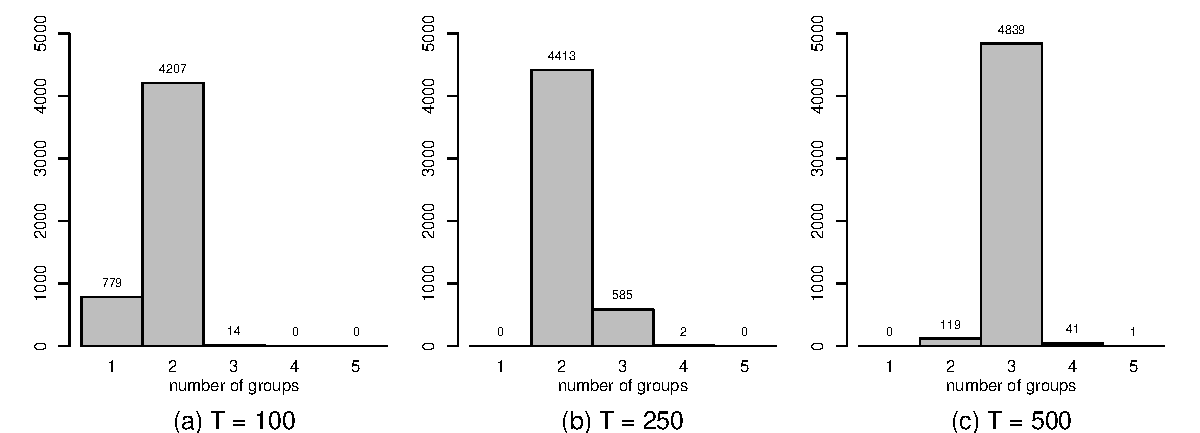
\includegraphics[width=0.95\textwidth]{output/plots/sim/histograms_groups}
%\caption{Estimated number of groups $\widehat{N}$ for nominal size $\alpha = 0.05$. 
%%Each panel corresponds to a different sample size $T$.
%}\label{fig:clustering:1}
%\vspace{0.25cm}
%
%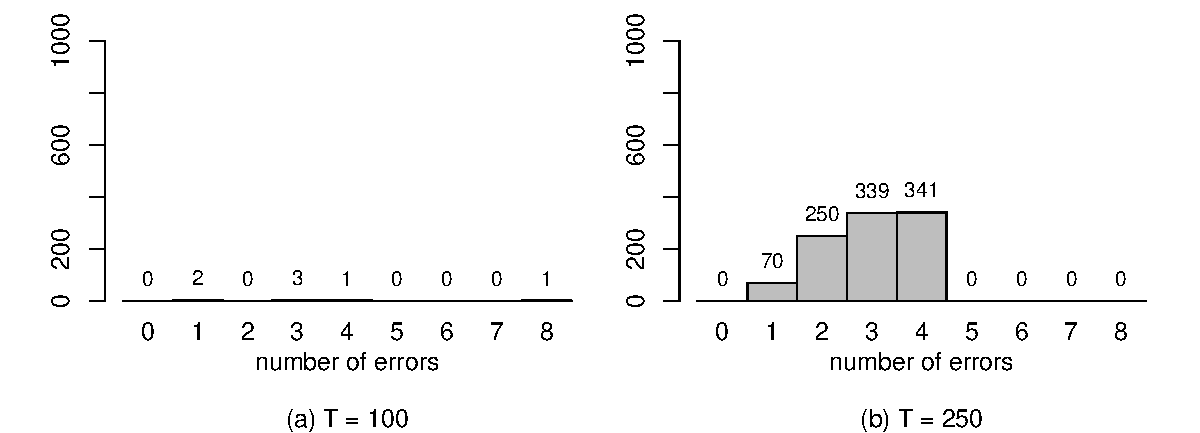
\includegraphics[width=0.95\textwidth]{output/plots/sim/histograms_errors}
%\caption{Number of classification errors for nominal size $\alpha = 0.05$. 
%%Each panel corresponds to a different sample size $T$.
%}\label{fig:clustering:2}
%\end{figure}

\textcolor{red}{Here we have a problem: the benchmark procedure is actually pretty good, much better than our method. It is very slow though. Discuss during the next call?}

The simulation results are reported as follows. For our multiscale method, the empirical probabilities with which which the estimate $\widehat{N}$ is equal to the true number of groups $N = 3$ for the significance level $\alpha=0.05$ for $T=100, 250$ and $500$ are $0.028, 0.117$ and $0.9678$, respectively. Furthermore, the  empirical probabilities with which the estimated group structure $\{ \widehat{G}_1,\ldots,\widehat{G}_{\widehat{N}}\}$ equals the true one $\{G_1,G_2,G_3\}$ for the significance level $\alpha=0.05$ for $T=100, 250$ and $500$ are $0, 0.1112$ and $0.9674$, respectively. The benchmark procedure is able to detect the difference between the groups in all possible case for all of the sample sizes. \textcolor{red}{There must be something wrong here, no?}

%in Table \ref{tab:clustering}. The entries in Table \ref{tab:clustering:1} are computed as the number of simulations for which $\widehat{N} = N$ divided by the total number of simulations. They thus specify the empirical probabilities with . Analogously, the entries of Table \ref{tab:clustering:2} give the empirical probabilities with which the estimated group structure $\{ \widehat{G}_1,\ldots,\widehat{G}_{\widehat{N}}\}$ equals the true one $\{G_1,G_2,G_3\}$. The results in Table \ref{tab:clustering} nicely illustrate the theoretical properties of our clustering algorithm. According to Proposition \ref{prop:clustering:1}, the probability that $\widehat{N} = N$ and $\{ \widehat{G}_1,\ldots,\widehat{G}_{\widehat{N}}\} = \{G_1,G_2,G_3\}$ should be at least $(1-\alpha)$ asymptotically. For the largest sample size $T = 500$, the empirical probabilities reported in Table \ref{tab:clustering} can indeed be seen to exceed the value $(1-\alpha)$ as predicted.% by Proposition \ref{prop:clustering:1}.For the smaller sample sizes $T=100$ and $T=250$, in contrast, the empirical probabilities are substantially smaller than $(1-\alpha)$. This reflects the asymptotic nature of our results %Proposition \ref{prop:clustering:1} and is not very surprising. It simply mirrors the fact that for the smaller sample sizes $T=100$ and $T=250$, the effective noise level in the simulated data is quite high.


%Figures \ref{fig:clustering:1} and \ref{fig:clustering:2} give more insight into what happens for $T=100$ and $T=250$. Figure \ref{fig:clustering:1} shows histograms of the $5000$ simulated values of $\widehat{N}$, while Figure \ref{fig:clustering:2} depicts histograms of the number of classification errors produced by our algorithm. By the number of classification errors, we simply mean the number of incorrectly classified time series, which is formally calculated as $\min_{\pi \in S_{\hat{N}}} \big\{ |G_1 \setminus \widehat{G}_{\pi(1)}| +|G_2 \setminus \widehat{G}_{\pi(2)}| + |G_3 \setminus \widehat{G}_{\pi(3)}| \big\}$ with $S_{\widehat{N}}$ being the set of all permutations of $\{1, 2, \ldots, \widehat{N}\}$. The histogram of Figure \ref{fig:clustering:1} for $T=100$ clearly shows that our method underestimates the number of groups ($\widehat{N} = 2$ in $4055$ cases out of $5000$). In particular, it fails to detect the difference between two out of three groups in a large number of simulations. This is reflected in the corresponding histogram of Figure \ref{fig:clustering:2} which shows that there are exactly $5$ classification errors in $3924$ of the $5000$ simulation runs. In most of these cases, the estimated group structure $\{ \widehat{G}_1, \widehat{G}_{2}\}$ coincides with either $\{ G_1 \cup G_2,G_3\}$,  $\{ G_1, G_2\cup G_3\}$ or $ \{ G_1 \cup G_3,G_2\}$. In summary, we can conclude that the small empirical probabilities for $T=100$ in Table \ref{tab:clustering} are due to the algorithm underestimating the number of groups.  Inspecting the histograms for $T=250$, one can see that the performance of the estimators $\widehat{N}$ and $\{ \widehat{G}_1,\ldots, \widehat{G}_{\widehat{N}} \}$ improves significantly, even though the corresponding empirical probabilities in Table \ref{tab:clustering} are still somewhat below the target $(1-\alpha)$.  

\textcolor{red}{As the benchmark procedure does not provide an estimate of the number of clusters $K$, I have also compared the results for the known number of clusters ($K=3$) for $T=100$ and the results are not better... We almost never detect the true grouping anyway.}

%Additionally, it is presumably also better to use bump functions rather than linear maps. For example, we could use 3 groups with (scaled versions of) the functions $g_1$, $g_2$ and $g_4$ from Figure 2 in Vogt \& Linton (2020, Multiscale clustering of nonparametric regression curves)
  


\end{document}
